%------------------------------------------------------------------------------
%	Template owner:
%------------------------------------------------------------------------------
%	Name					: Harshad Sharad Sinkar
%	University				: Chemnitz University of Technology
%	Major					: MSc. Embedded System	
%	Matr. No.				: 424589  
%	Department			: Department of Computer Science  
%	Betreuer				: Prof. Dr.-Ing. XXXXX
%	Prüfer					: Prof. Dr.-Ing. XXXXX
%	Ausgabedatum		: XX.YY.ZZZZ
%	Abgabedatum		: XX.YY.ZZZZ
%------------------------------------------------------------------------------
%	Company Name	: Bosch Engineering Group (BEG), Abstatt
%	Department			: IoT-Embedded Linux (BEG/PJ-IoT-EL)
%	Betreuer 				: Prof. Dr.-Ing. XXXXX
%------------------------------------------------------------------------------
%------------------------------------------------------------------------------
\documentclass[a4paper, 12pt, oneside, BCOR1cm,toc=chapterentrywithdots]{scrbook}

\usepackage{graphicx}           % use for pdfLatex
\usepackage{makeidx} % f\"{u}r Benutzung des Befehls \printindex
\usepackage[colorlinks=false]{hyperref}
\usepackage{tocbibind}
\usepackage{listings}
\usepackage{blindtext}
\usepackage{subfigure} 
\usepackage{acronym}
\usepackage{tabularx}
\usepackage{afterpage}
\usepackage{textcomp}
\usepackage{hyperref}
\usepackage{listings}
\usepackage{enumitem}
\usepackage{lmodern}  % for bold teletype font
\usepackage{amsmath}  % for \hookrightarrow
%\usepackage{xcolor}   % for \textcolor
\usepackage{float}
\usepackage[dvipsnames]{xcolor}
\usepackage{fancyvrb}
\usepackage[titletoc]{appendix}
\hypersetup{%
bookmarksnumbered=true, hyperindex=true,
%
%Im Acrobat Reader Subtitel 1. Ebene anzeigen
bookmarksopen=true, bookmarksopenlevel=1,
%
pdfborder=0 0 0 % Keine Box um die Links!
}


%------------------------------------------------------------------------------
% Force Tables and List to be added in Table of Content
%------------------------------------------------------------------------------

\renewcommand*{\tableofcontents}{%
  	\begingroup
  	\tocsection
  	\tocfile{\contentsname}{toc}
  	\endgroup
}
\renewcommand*{\listoffigures}{%
  	\begingroup
  	\tocsection
  	\tocfile{\listfigurename}{lof}
  	\endgroup
}
\renewcommand{\listoftables}{
	\begingroup
	\tocsection
	\tocfile{\listtablename}{lot}
	\endgroup
}
\newcommand\blankpage{%
    \null
    \thispagestyle{empty}%
    \addtocounter{page}{-1}%
    \newpage}   
  
\lstset{
	basicstyle=\ttfamily,
	columns=fullflexible,
	frame=single,
	breaklines=true,
	postbreak=\mbox{\textcolor{red}{$\hookrightarrow$}\space},
}  


\begin{document}
%------------------------------------------------------------------------------
%------------------------------------------------------------------------------
%
%  Here I go . . .
%
%------------------------------------------------------------------------------
%------------------------------------------------------------------------------

%--------titlepage
\begin{titlepage}

{
    
    %\begin{center}
        %\raisebox{-1ex}{
\includegraphics[scale=1.5]{TU_Chemnitz_positiv_gruen.pdf}}\\
    %\end{center}
    \begin{center}
    
	\raisebox{-.4\height}{
\includegraphics[scale=.5]{images/BEG_Logo.jpg}}\raggedleft
	\hfill
	\raisebox{-.4\height}{
\includegraphics[scale=0.8]{images/TU_Chemnitz_positiv_gruen.pdf}}\raggedright
	
    \end{center}
}


\begin{center}

\LARGE{\textbf{Learning Based Performance Prediction For Embedded Hardware}}\\
\vspace{0.8cm}


\Large{\textbf{Master Thesis}}\\ 
\vspace{0.8cm}
Submitted in Fulfillment of the\\
Requirements for the Academic Degree\\
M.Sc. Automotive Software Engineering\\
\vspace{0.5cm}
Dept. of Computer Science\\
Chair of Automotive Software Engineering\\
Technische Universit{\"a}t Chemnitz, Germany\\
\vspace{0.5cm}
Thesis work carried out at Software Systems Engineering Dept., Robert Bosch GmbH, \\
Renningen, Germany

\vspace{0.8cm}
	\begin{tabular}{@{}>{}rl@{}}
			Author:	& Rahul Gajanan Mahajan \\
    		Student ID:	& 424592               \\
    		Supervisors:	& Dr. Arne Hamann \\
    						& Michael Pressler \\
    						& Falk Wurst \\
    		Examiner:	& Dr.-Ing. Alejandro Javier Masrur\\
    					
  	\end{tabular}

\vspace{0.5cm}  	
\today\\  	

\end{center}
\end{titlepage}

%------------------------------------------------------------------------------
% Blank Page
%------------------------------------------------------------------------------
\afterpage{\blankpage}

%Here starts the real work
%------------------------------------------------------------------------------
% Acknowledgement
%------------------------------------------------------------------------------

\addchap*{Acknowledgement}
\addcontentsline{toc}{chapter}{Acknowledgement}
% ------------------------------------------------------------------------------
% Acknowledgement
% ------------------------------------------------------------------------------
\setlength{\parindent}{4em}
\setlength{\parskip}{1em}

I am grateful for all support and encouragements toward me during my master thesis at Robert Bosch GmbH. First, I would like show my gratitude to Prof. Dr.-Ing.  Alejando Masrur for giving me an opportunity to perform my master thesis under his guidance and  and giving freedom, support and suggestions in every phase of my thesis development. 

\par I am eternally grateful to my supervisors at Robert Bosch, Dr. Arne Hamann, Michael Pressler and Falk Wurst for giving me an opportunity to work on such a interesting topic of master thesis. I am thankful for their time, patience and continuous support during my entire period of thesis. It was great privilege and honor to work under their guidance. I would like to thank them for motivating me at every of phase of thesis and providing me ideas during thesis work. It was very great journey working with Software System Engineering department at Robert Bosch, I would like to thank all my other colleagues contributed during my thesis work.  

\par I would also like to thank my parents and all my friends who kept supporting me in my tough time and helped me. 

%------------------------------------------------------------------------------
% Abstract
%------------------------------------------------------------------------------

\addchap*{Abstract}
\addcontentsline{toc}{chapter}{Abstract}
% ------------------------------------------------------------------------------
% Chapter 00 : Abstract
% ------------------------------------------------------------------------------
\setlength{\parindent}{4em}
\setlength{\parskip}{1em}

Due to market pressure, software and hardware are developed together. But sometimes the hardware is in prototype phase or not yet have been developed yet. In such cases, it is hard to get performance of software on hardware which may be unavailable during development phase. To address this issue cycle accurate simulators are used to get the performance of software. But there are challenging problems with these simulation tools, they are often slow and expensive. 

\par In this thesis work, we propose the learning based approach that synthesize the analytical models that can accurately predict the performance of software for hardware platform.  We apply a fine grained phase based approach, where learning algorithm predict the performance of the software workload. All performance aspect data using hardware performance counters of processor, is collected for software workload on hardware platform at phase level and given to learning algorithm to predict the performance at phase level of software workload.

\par Learning approach relies on a one time training data collected at different granularities. We used software programs from ACM-ICPC and Sanfoundry to collect the training data. We applied our approach on 9 benchmarks from MiBench benchmark suite. 

\par Results shows that average over 86\%  prediction accuracy for fine grained performance. 

%------------------------------------------------------------------------------
% Table of Contents, List of figures, List of Tables
%------------------------------------------------------------------------------

\tableofcontents
%\listoffigures
%\listoftables

\onecolumn
%------------------------------------------------------------------------------
% Chapter 1 : Introduction
%------------------------------------------------------------------------------
\chapter{Introduction}
% ------------------------------------------------------------------------------
% Chapter 1 : Introduction
% ------------------------------------------------------------------------------
% parameters setting
\setlength{\parindent}{4em}
\setlength{\parskip}{1em}

This thesis evaluates approach of estimating the performance of software workload on embedded hardware using machine learning. This is achieved by researching different available techniques, approaches and tools to evaluate performance of software on embedded hardware processor. This work is an attempt to represent the relevant features and highlighting various factors in existing methodology. 


\par Now a days electronic systems are widely used in automotive industry. These electronic systems provide better control than mechanical control with use of the software. These systems are used in commercial vehicles, trucks, motorcycles, forklifts, tractors, excavators and many more automobiles. And these electronic systems provide better control to and collect information from automobiles. These systems consist of electronic components such as processors, sensors, actuators, electrical components, electrical circuits, communication devices, power supply units and others. 

\par Electronic systems provide control operations in different domains of vehicles such as powertrain, chassis, passive safety, body/comfort, multimedia/telematics and man-machine interface which consist functionality like engine management, gearbox control, anti-locking system, electronic stability program, airbag control, navigation,instrument panel and many more. All these domains are connected and communicate to each other through on board electronic bus systems techniques such as Controller area network(CAN), Media oriented systems transport(MOST), etc.

\par In automotive electronics systems, Electronic control unit(ECU), is embedded system provides control to one or more electrical systems or subsystems in vehicles. ECU consist processors, interface for inputs and outputs, memory, communication links and many more. All sub domains discussed above consist one or more ECU as electronic system. Now a days upto 80 ECUs are used in modern cars. Development of ECU involves hardware and software to execute tasks for defined module. ECUs are programmable and can be reprogrammed according to functionality and requirements. Now a days, ECUs have more computing powers in single processor. Modern days processors provide higher computing powers typically upto 64 bit processing and operating frequency in gigahertz. Following figure \ref{fig:ecu} illustrate the ECUs used in various domains of a vehicle. Automotive electronic control unit market predicted to reach upto \$55.97 billion by 2024. Around 40\% of revenue in automotive industry is from automotive electronics. This is because most of vehicles are software driven[ref].

\begin{figure}[h!]
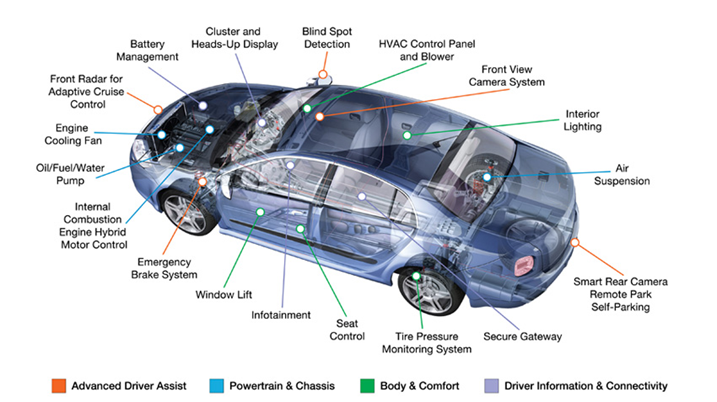
\includegraphics[width=12cm, height=8cm]{./images/ecus_in_car}
\centering
\caption{Number of ECUs are used in different domains of single vehicle}
\label{fig:ecu}
\end{figure}

\par Software is an integral part of embedded system in automotive domain. Software is running on microprocessors/microcontrollers provides the control mechanism. It is brain behind the every action taken in embedded systems. In current era, software is backbone for advanced features used in automobiles such as advance driving assistant systems have anti-breaking systems(ABS), electronic stability program(ESP), parking assistance system and many more. It also perform measure role in safety critical system used in automobile. As software plays important role in embedded systems then performance of software is also essential. Performance of software in application of safety critical systems is not only needed to be correct but also should have quick repose time. So performance of any software running on embedded hardware need to be evaluated before integrate with real hardware and used in application. 

\par Software performance is not only about how fast it can handle large numbers but it is also about memory management, networks, cores, architectures. Some algorithms looks good on paper but they perform poorly on hardware. Being able to manage the performance of software requires well understanding of hardware architecture, operating systems and runtime libraries[ref- lemire.me].  As mentioned above, modern cars have more than 70 ECUs per vehicle.  Following figure \ref{fig:num_ecu} shows increase in the number of ECUs year by year in automotive industry. Each ECU has number of functionalities to perform. Year by year number of ECUs per vehicle are increasing and ability to perform functionalities per ECU is also increasing. According to Moore's law, number of transistors on integrated circuits doubles approximately every two years. This advancement in capabilities of a ECU is due to growth in technology of semiconductor manufacturing as well as demand of software driven vehicles.  

\par Each ECU in vehicle has it's own software stack to control the operations, diagnostics, monitoring the network, reading the sensor values, to operate the actuators and many operations. In demand of software driven vehicles software performs the crucial part in it. Whether it is safety critical systems, powertrain system, advance driving assistance systems, multimedia systems in vehicle. All these systems have their own ECUs which controlled by software. In world of competition, each original equipment manufacturers and suppliers wants to stay ahead of each other and they are coming with new features and technology in the automotive industry. In current trade of automotive industry and future of automotive industry, interest in software driven vehicle is increasing and it is expecting improvement in hardware which can deliver the adequate performance of software. Software is playing the vital role of performance of vehicle as well as in automotive industry.

\begin{figure}[h!]
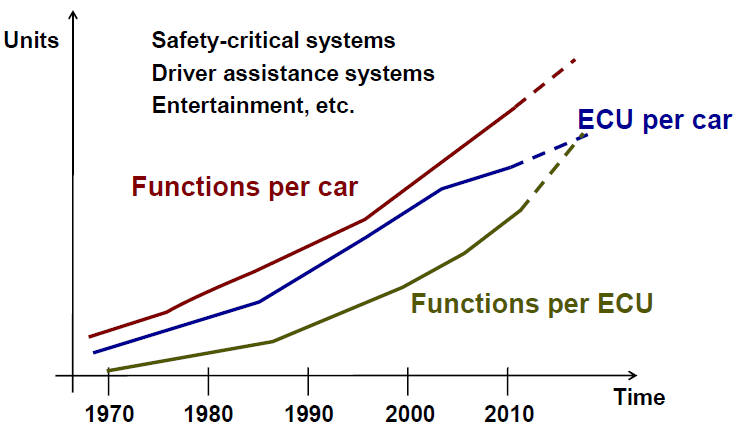
\includegraphics[width=12cm, height=8cm]{./images/ecu_per_year}
\centering
\caption{Trends in automotive systems}
\label{fig:num_ecu}
\end{figure}


\section{Purpose of the Thesis Work}
In initial phase of the thesis work, we discussed the problems behind the product development with sequential method and effect of the market pressure to release the product. Also tools available in market to evaluate the performance of software.

\subsection{Sequential development}
In automotive industry, sequential product development model is used widely to develop a product. V-model is one the broadly used process to develop a product. V model is also known as verification and validation model and processing is performed in V-shape. You can see in following figure \ref{fig:v-model} the V-model design.

\begin{figure}[h!]
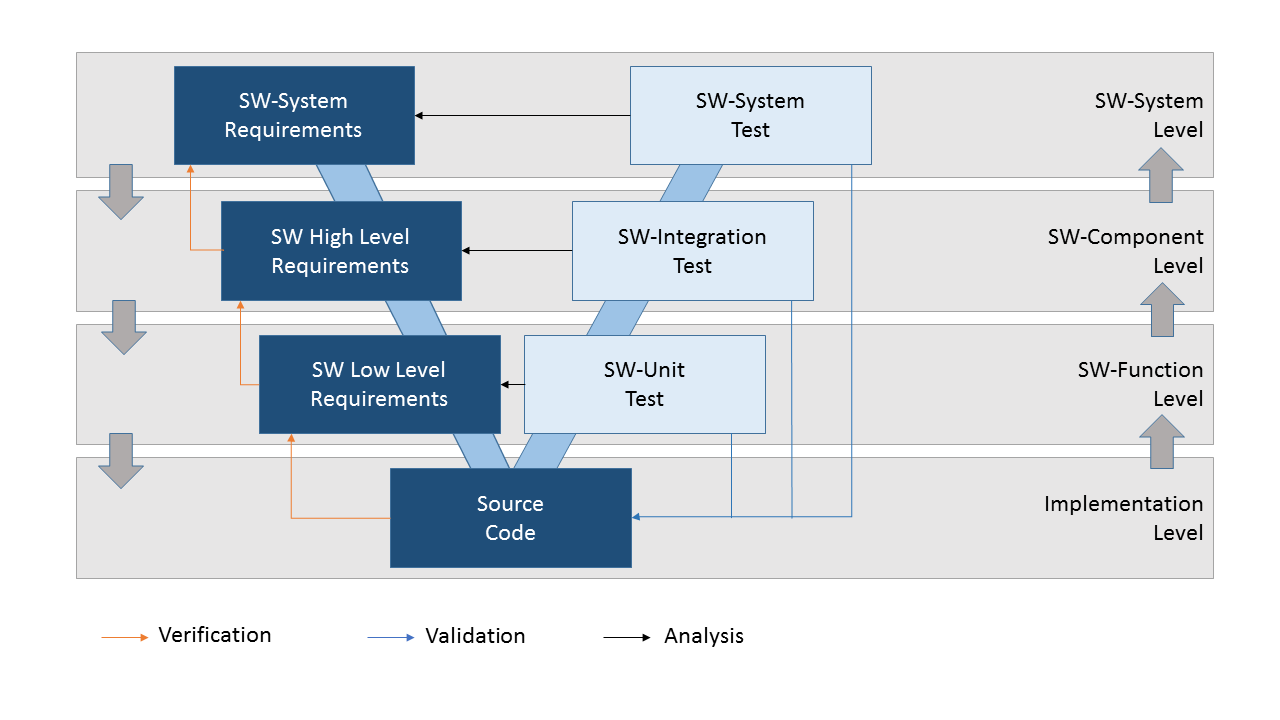
\includegraphics[width=14cm, height=14cm]{./images/V-Model}
\centering
\caption{V-Model}
\label{fig:v-model}
\end{figure}


\par To give small overview of V-model, it starts with requirement phase. Where customers and OEMs provide their product requirements. After that hardware and software architecture requirements are carried out and then process go to much more detail. In next phase component level requirements are collected and analyzed. After all high level and low level requirements, implementation process starts. After implementation, different testing techniques are performed at each corresponding phase, to identify bugs in low level, high level and system level design and implementation of product. And after all this final product is delivered to customer or OEMs.

\par Sequential development where software development waits for available hardware, is still prevailing industry norm. And this flaw of sequential development method is that to implementing software for product, hardware requirement must be known to software developers. Software developers need hardware architecture, memory, input/output(I/O) and many more parameter to design the architecture of software. After building the software for given hardware architecture and product, software tester need to test it on hardware and which should be available to testers. In some cases this hardware dependencies are observed and it delays the product release to customer, OEMs or to market. 

\subsection{Parallel development}
For every product development, time, cost and quality, these are key concerns. In device supply chain of semiconductor companies and OEMs are turning to parallel product development to shorten the development cycles and buy time to integrate  and test products. Virtual prototypes are used in parallel development, where virtual prototypes are functional software model of systems under development. These virtual prototypes are used in unavailability of harware, which helps faster software development. 

\begin{figure}[h!]
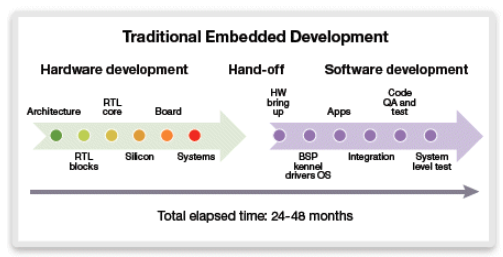
\includegraphics[width=12cm, height=7cm]{./images/seq_dev}
\centering
\caption{Time estimation for sequential product development}
\label{fig:seqn_dev}
\end{figure}

\par Embedded devices mostly depends upon custom hardware. These devices have broad array of use cases and hence they give rise to broad array of hardware architectures. There is no standardize platform is available. Absence of standardization increases  the time in product development. As mentioned in this [ref], realistic time estimation to develop complex embedded project requires 36 to 48 months of time with sequential development method.  12-18 months to hardware development, and 12-18 months for software development and 6-12 months for integration, verification and validation. Above figure\ref{fig:seqn_dev} illustrates the estimate time to build product using sequential method.

\par As we seen in above figure \ref{fig:seqn_dev}, software development lies on right hand side. And shifting left the software development process with parallel to hardware development results in parallel development. It can be seen in following figure \ref{fig:par_dev}. In parallel development, hardware and software team work in lock-step, communicating regularly, and continuously integrating hardware and software results into save time for modifications. With use virtual prototype tools parallel development of product can be possible. 

\begin{figure}[h!]
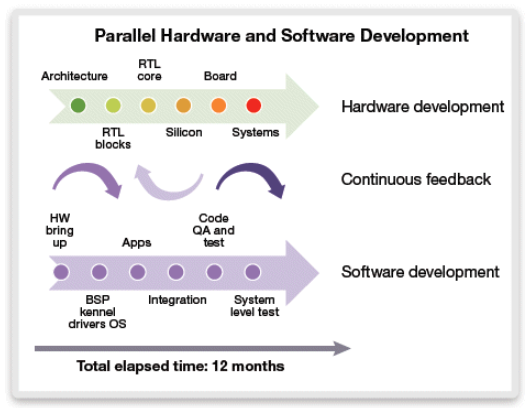
\includegraphics[width=12cm, height=10cm]{./images/par_dev}
\centering
\caption{Hardware and software development in parallel}
\label{fig:par_dev}
\end{figure}

\par In some scenarios, the system(s) on chip(SoC) takes time to come back from fabrication. In such scenarios, using virtual prototype of same SoC, software development can moves forward. It gives time to software developers for debugging and testing. With use of virtual prototypes in parallel development, avoid delays in product development as well as in product release in market. 

\section{Motivation}
Advanced risc machine(ARM), is family of reduced instruction set computing(RISC) architectures for computer processors. Arm holdings develops architecture and licenses it to other companies, who design their SoC product that includes architecture provided by ARM incorporate with memory, interfaces and many more. Processor architectures made by ARM are widely used automotive industry to develop ECUs as well as in other consumer industry for electronic products. ARM also provides the solutions for virtual prototyping, which provides motivation to my thesis work. Also it provide development solutions to embedded systems and servers. These tools are used in development od billions of ARm-based devices on the market.

\par As previously discussed how virtual prototypes help in early software development independent to physical availability of hardware. Goal of the ARM is to provide pre-silicon software development and analysis with better analysis, accuracy, availability, performance and ease of use. Following diagram \ref{fig:arm_dig1} illustrates available virtual prototypes/simulators from ARM with respect to abstraction level and simulation speed.

\begin{figure}[h!]
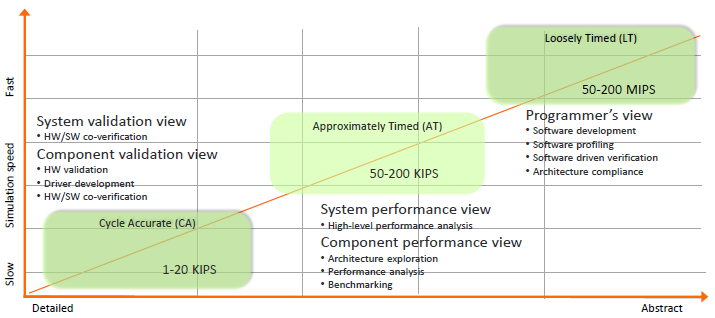
\includegraphics[width=14cm, height=10cm]{./images/arm_dig1}
\centering
\caption{ARM virtual prototype solutions}
\label{fig:arm_dig1}
\end{figure}

\par In above diagram \ref{fig:arm_dig1} ARM has cycle accurate tool which provides detailed abstraction level but slow simulation speed in between 1-20 kilo instructions per second(KIPS). This tool can be used for system validation and component validation applications such as hardware/software co-verification, hardware validation, driver development. This cycle accurate tool is known as ARM cycle models. ARM also provide loosely timed tool for simulation of SoCs. Which does not need detailed abstraction level and provides high simulation speed witn 50-200 million instructions per cycle(MIPS). This loosly coupled tool is known as ARM Fast Models. It can be used for application like software development, software profiling, and software driven verification.

\par Above diagram \ref{fig:arm_dig1} shows that for detailed abstraction level ARM cycle models can be applied but it provide slow simulation speed. Whereas ARM fast models can be applied where high simulation speed and not detailed abstraction level required. But there is no tool available where intermediate simulation speed and abstraction level required. For targeted application such as software profiling, benchmarking, performance analysis and software development. All these tools are expensive and also sometimes project dependent. And this problem motivates me to perform my research in my master thesis and find the optimal solution.

\par Performance of software, running on hardware can be measured.  Using machine learning it is possible to learn the performance relevant aspects of hardware platforms (SoC) to be able to predict the timing behavior of different applications. Performance of software running hardware can be measured in terms of micro-architectural events. Now a days every processor comes with hardware performance counter to monitor micro-architectural events. By running different software applications on two embedded cross platform hardware, statistical relationship can be formed and using this relationship can be use to predict the performance of software using machine learning. 

\subsection{Outline}





  % Load Data from File intro.tex
%------------------------------------------------------------------------------
% Chapter 2 : State of the Art
%------------------------------------------------------------------------------
\chapter{State of The Art}
% ------------------------------------------------------------------------------
% Chapter 2 : State of the Art
% ------------------------------------------------------------------------------
\setlength{\parindent}{4em}
\setlength{\parskip}{1em}
\section{What is Performance?}
Performance of any embedded system is depends upon the amount of the work accomplished by it and it depends upon many context. Performance depends upon many aspects. One of the aspect is response time, it is total time taken by system to respond the service being requested. Another aspect maybe processing speed, how many instructions are processed at a time provides the processing speed of the system. High throughput for input and output data, bandwidth, power consumption, latency, availability and many aspect are there for performance. In this thesis our main performance aspect is total number of cycles to execute the software at different phases.  


\par There are many techniques and tools are available to observe the performance of software on given embedded hardware. Some of these techniques are provided by tool vendors and some of them are part of industrial and educational research. Using tools provided by vendors, which helps to analyze the performance data graphically and provide more functionality and features to software engineers. Such tools are Silexica[link], ARM Streamline Performance Analyzer[link], or hardware simulation tools such as gem5 simulator[link to gem5]. Also there are ongoing research to evaluate the performance of software using machine learning techniques with state of the art. Using machine learning technique, it is possible to predict the performance of software by creating dataset of performance. Also using Worst Case Execution Techniques[WCET] use to analyze the performance.

	\par Traditional simulation approaches, simulator estimates the performance of software or application running on slow cycle accurate or cycle approximate models ISSs [1.3,2.7] of target embedded hardware processor. To improve the speed of ISSs and maintain the accuracy, hardware-assisted acceleration and transaction level techniques are recently proposed [2.5,2.8]. Chiang et al. [ieee] discusses the fast cycle accurate ISS for SoC based on QEMU and system C.  Li et. al[IEEE] discusses the inspection of problem to determine the WCET of processor. This paper further discuss issue of micro-architectural modeling to determine the WCET of known instruction sequence. Without need of source code or reverse engineering on binary files,it is possible to estimate WCET for software or application using integer linear programming(ILP) and constraint logic programming(CLP)[ieee]. Analytical model to estimate the performance of software on cross platform with using learning based techniques is discussed by Gerstlauer et. al [IEEE]. It evaluates the performance prediction of whole program using regression learning technique. Further they added new methodology[ieee] using learning model, to predict the power and performance of software at different phases of software or applications. Using analytical techniques, Joseph et.al [] obtains good approximate model Akaike's information criteria is used in iterative process to extract a linear model. Lee et al. [1.18] and Khan et al [1.14] focused on predictive modeling approach from uni-processor to multi-processor and multicore proccessor. 

\section{Analytical Models}
Analytical models are models which contains the information about behavior of system. It has data regarding input and output the system. Using this data which tell the behavior of system is used to form mathematical model or statistical model to understand the system. This analytical models are learned using learning algorithm techniques. There are different techniques to evaluate the performance of software on hardware by creating analytical models. Following are the state of the art performance analytical models used to predict the performance of software on processor.

\subsection{Learning-based Analytical Cross-Platform Performance Prediction}
This IEEE paper published by Gerstlauer and his colleagues from University of Texas at Austin, USA. This paper focuses about challenges with cycle accurate simulators and how analytical models is used to get performance evaluation of software at higher speed.

\par Simulation based models are widely used to model the hardware but these models are costly as well as slow to evaluate the performance of software using micro-architectural events. As collection of performance data on ISS is slow but collection of performance data on existing platform is faster because execution is done at native speed. Latent relationship can obtain by executing a program of processor and executing the same program of different processor. In this paper 'target' is preferred as platform for which the prediction is performed and 'host' is preferred as platform for which various statistics are collected. Host platforms are AMD Phenom II X6 1055T and Intel Core i7 Core. Target is platform is ARM processor model simulated on gem5 simulator.  

\par Performance of software on target and host platform is measured using performance evaluation tool PAPI. PAPI measures all micro-architectural events from PMU with respect to software executing on hardware platforms. In this scenario, performance aspect is number of cycles consider. Total 157 programs with and 100 instances for each program are used to collect the training data. Input vector for Intel and AMD are different in term of number. Because number of performance counter supported by both processors are different. Intel i7 supports 14 where as AMD Phenom supports 8 hardware performance counter using PAPI. Training data collected from both host platform excepting the total cycles. total cycles event is collected on gem5 simulator for ARM processor for same 157 programs and 100 instances. Training data help to understand this relationship between input feature vector and output feature vector. Following figure \ref{fig:paper1} shows the framework for this paper. 

\begin{figure}[h!]
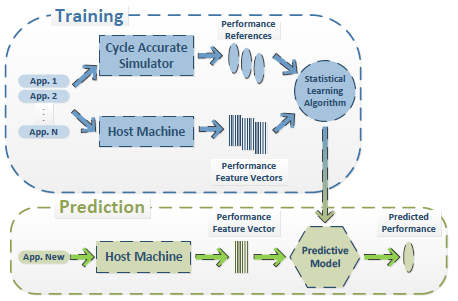
\includegraphics[width=12cm, height=8cm]{./images/ieee1}
\centering
\caption{Cross-platform performance prediction framework[]}
\label{fig:paper1}
\end{figure} 

\par To understand the collected training data, data is visualized using data analysis and data visualization techniques such as Principal Component Analysis(PCA) for reduce the dimensions and Co-relation coefficient for one to correlation of hardware performance counters. Using learning techniques this statistical model is learned and prediction is performed. Regression technique of machine learning is used. In which Lasso linear regression and Constrained Locally Sparse Linear Regression(CLSLR) are used. To select the best learning model cross-validation technique is used and as best result CLSLR is preferred. 

\par To test the accuracy of CLSLR algorithm,accuracy test is conducted on 15 different programs which are not used during training data collection. Input feature vectors for all these test programs are collected on both platforms. Result for predicting the whole program performance, errors of more than 40\% are observed on embedded benchmarks. 

\subsection{Accurate Phase-Level Cross-Platform Power and Performance Estimation}
This IEEE paper is also published by Gerstlauer and his colleagues from University of Texas at Austin, USA with improved and additional features with respect to previous paper. In this research, authors provided LACross method learning based method, for cross-platform time varying software performance as well power consumption predictions. Where all data is collected with fine-grained phase based approach. Also instead of simulation model, native hardware platforms are used for target and host.

\par In this approach host platform is Intel i7 920 processor used. Whereas as target platform, ODROID-U3[ref] development board is used which contains ARM Cortex-A9 processor and to collect the power consumption ODROID-XU3 development board is used with on-chip TI IN A231 current sensor. To collect training data, similar programs are used as it mentioned in previous paper except 100 instances, here only single instance is used. Training data collected on these hardware platform using performance evaluation tool PAPI. Feature extraction for host platform contains all hardware performance counter except cycles where as feature extraction for target hardware are total cycles and power consumed. Following diagram illustrate the framework for LACross. It has similar goal is to accumulated latent relationship between to processor.

\begin{figure}[h!]
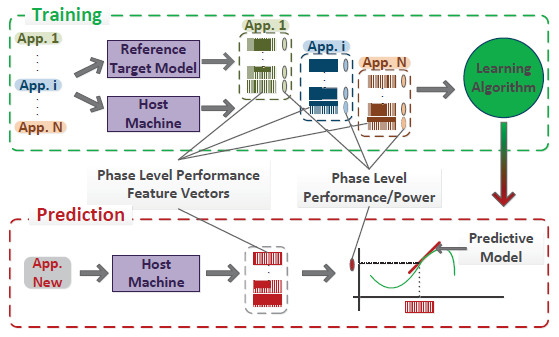
\includegraphics[width=12cm, height=8cm]{./images/ieee2}
\centering
\caption{LACross overview[]}
\label{fig:paper2}
\end{figure}

\par All these features are extracted using LLVM tool chain. Where LLVM uses Clang as compiler and it interfaced with PAPI libraries to collect the data at different phases of software. Time varying performance of software on hardware platform is collected in database. Values of performance counter is measured at each phase of software by inserting PAPI API calls to provide time varying data. 

\par All training data is gathered from host and target platform applied to learning algorithms. In this paper, variant of Lasso regression, that is Simplex Constrained Quadratic Programming(SCQP) applied to predict the performance and power consumption of software on hardware platforms at each phase level. All results are calculated on 
35 selected benchmark programs from three different standard benchmark suites. All these benchmark programs are not included during the training data collection phase. 
Results shows over average 97\% accuracy for both performance and power consumption at higher speed of 500 MIPS. 

\subsection{Composable Performance Regression for Scalable Multiprocessor Models}

\section{WCET analysis}
\subsection{Combining instruction set simulation and WCET analysis for embedded software performance estimation}

\section{Silexica}
Silexica GmbH provides tools for software design automation which enables software developers and system architecture to design and program multicore systems via SLX tool suite. System architects work with software models which maybe open source, in house, commercial source, the traditional methods are not scalable for software optimization in multicore system. To understand the software or system behavior on multiocre system, a full and precise analysis of software interdependencies are required. So a tool is need to give deep insights on software interdependencies that occur during execution on multicore system. SLX is multicore development tool that provides software execution insights into hardware and software interdependencies.It allows for code architecting and refactoring to achieve the most efficient utilization of CPU, DSP, FPGA and other acceleration engines on multicore systems[].

\par SLX also can be use for software/hardware exploration. Current generation tools are not able to provide exploration to today's complex heterogeneous SoCs. These SoCs are big unimaginable challenges with present available tools. In current market of SoCs, SoCs with increasing number of cores, acceleration engine, decreasing the chip size are available in lower cost and high performance with less power consumption. In such wide varieties of SoCs, it is more challenging to fing optimal target platform for developing application. To select correct SoC for application requires clarity of software and hardware interaction. This interation can be useful to minimize disagreement and maz=ximize the performance. 

\par SLX features behavioral model for modeling multicore SoCs which made of co-processors, graphical processing units(GPUs), field programming gate arrays (FPGAs), communication buses, inter-connectivity, memory hierarchy and clusters. SLX system models provide rapid profile change with respect to hardware variance to facilitate hardware investigation for application software. SLX is able to predict the system behavior and memory performance based on simple and high level application model.

\par SLX analyze behvior of multiple application on target platform  and calculate the intercommunication delays. It also provides static and dynamic source code analysis, data and control dependencies. SLX also provide optimization to optimize the distribution of application to hardware and identification of blocking dependencies and control. Optimizations are driven by performance, power, and memory requirements for given combinations of FPGAs, GPUs and cores.  SLX support multiple programming languages to create high level application from scratch directly from your source code. It also support command line interface on windows and linux platforms. 

\par Silexica provides wide range of hardware platforms to analyze the behavioral of application software on different hardware platforms by measuring computing power, inter-connectivity, number of cores, delays and many more factors. It support software developers to understand the behavior of application on hardware platforms which may not be available in market or in still in prototype phase.   % Load Data from File intro.tex
%------------------------------------------------------------------------------
% Chapter 3 : Design and Implementation Storyboards
%------------------------------------------------------------------------------
%\chapter{Setup Steps and Basic Usage Insight}
%% ------------------------------------------------------------------------------
% Chapter 3 : Setup steps and Basic Usage Insight
% ------------------------------------------------------------------------------
\setlength{\parindent}{4em}
\setlength{\parskip}{1em}

In this section we will go through basics like performance measurement concept, tools to measure performance, LLVM, instruction set simulator(ISS) and basic learning techniques to understand the thesis. Performance of software on embedded hardware is essential in embedded product development. The measure question is how to measure performance of software on hardware. Here software maybe an application or operating system. Performance of application or operating system can be  analyzed and improved using performance monitoring features provided by embedded hardware. Now every modern hardware processor has Performance Monitoring Unit(PMU) on chip. PMU is on-chip hardware device that monitors the micro-architectural events. Events like cache hits, cache miss, cycles etc. Data collected from PMU can be use to observe the behavior of application or operating system on hardware processor. This collected data can be use to improve the performance. 

\par Performance monitoring events can be categorized in two types, one is hardware events and second is software events. Hardware events contain the events related to hardware like cycles, instructions, cache miss, cache hit etc. Where software events are related to software like page fault, segmentation fault, context switch etc. Performance monitoring hardware consists two components, performance event select registers and event counters. Performance event select registers are configuration registers to control what events to be monitored and how to monitor. Event counters registers, those count the number of events based on event select registers configuration. Also there are two approaches for performance monitoring, one is counting and other is event based sampling. Following figure \ref{fig:pmu} shows the block diagram of PMU in ARM Cortex A53 processor. 

\begin{figure}[h!]
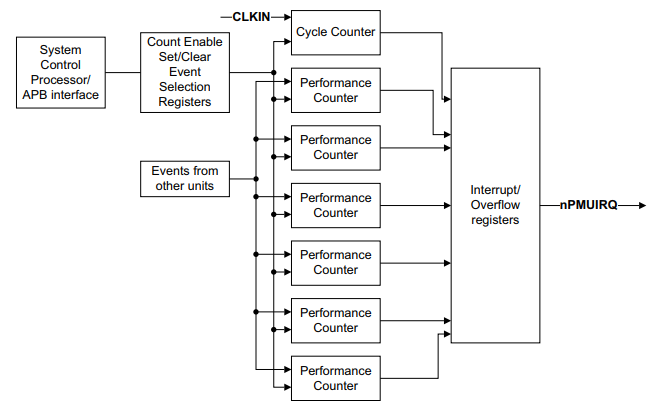
\includegraphics[width=14cm, height=10cm]{./images/pmu}
\centering
\caption{Block diagram of PMU in ARM Cortex A53 processor}
\label{fig:pmu}
\end{figure}

\section{Tools for Performance Measurement}
To evaluate the performance of software on hardware, variety of tools are available. These tools provide high level interface and analysis capabilities for performance monitoring hardware. The Performance Application Programming Interface (PAPI) tool suite [papi link] provides a common interface to performance monitoring hardware for many different processors like Alpha, ARM, MIPS, Pentium, PowerPC and etc. VTune Performance Analyzer [link for it] from Intel support performance monitoring on Intel's processor. PERF is performance analyzing tool in Linux, available from Linux kernel version 2.6.31 [link for perf]. OProfile[link for OProfile] is system-wide  statistical profiling tools for Linux to measure the performance of underlying hardware processor. ARM's Streamline Performance Analyzer provide in depth look of software performance on ARM processors. In this thesis, we are going to see tools like PAPI, PERF and Streamline Performance analyzer to evaluate the performance of software. In this thesis, we are focusing on hardware events and the performance data provided by these performance measurement tools measured on Raspberry Pi 3B board, which includes ARM Cortex A53 processor.

\subsection{PERF}
PERF is performance analyzing tool in Linux operating system and it is available from version 2.6+ of Linux kernel. PERF can accessed by userspace controlling utility, named 'perf'. PERF command line interface on Linux provides number of subcommands. PERF provides statictical data performance data of Linux kernel and user application. PERF supports hardware performance counters, software performance counters and tracepoints. PERF is based on 'perf\_events' interface. 

\par PERF Linux tool supports wide majority of events to provide the performance data. This tool can measure events from different sources using kernel interface. One source of events are kernel counters and these events are called software events like context switches, page-fault, alignment fault, emulation fault and etc. Another source of events is processor itself. PERF reads the events from hardware performance counter of PMU of processor. PERF provides the list micro-architectural events supported by it such as number of cycles, L1 cache miss, total instructions, branch mispredicted and many more.  Finally, the tracepoint events which are provided by kernel through 'ftrace' infrastructure.

\par One of the main feature of the PERF is that it allowed to select the specific core/s of processor using processor-wide mode. The performance data of specific core/s  can be collected for given application or operating system. Which had very significance in this thesis. It also creates the report of the collected sample data in file called 'perf.data'.It also possible with PERF to go more in granularity of instruction level with 'perf annotate'. 	PERF also provide the live analysis like Linux top command with processor wide feature. it is possible to measure the performance of application in userspace as well as kernel space. 

\par PERF provides subcommands on command line interface such as 'stat, record, report', etc. It is possible to get the list of software and hardware events supported by PERF using 'list' command for running embedded hardware processor. Following is the PERF usage on Raspberry Pi 3B board with Raspbian, Linux based operating system and we are measuring the performance of basicmath application from Mibench suite[] for single core i.e. second core of Cortex A53..


\begin{lstlisting}
$ sudo perf_3.16 state -e cycles,instructions,cache-misses,
 branches,branch-misses -C 2 ./runme_large.sh

# started on Wed Apr  4 14:02:59 2018 

Performance counter stats for 'CPU(s) 2':     
1,654,827,425      			cycles                        
1,397,787,969      			instructions              #    0.84  insns per cycle                    
3,528     	 				cache-misses                                                       
94,047,959     	 			branches                                                             
2,669,120    	 			branch-misses          #    2.84% of all branches              
2.445278109 seconds time elapsed
\end{lstlisting}

\subsection{PAPI}
PAPI is abbreviation for Performance Application Programming Interface. PAPI project is developed at University of Tennessee's Innnovative Computing Laboratory in Computer Science Department. This project was created to design, standardize, and implement a portable and efficient Application Programming Interface (API) to access the hardware performance counters found on most modern microprocessors[papi user guide]. PAPI provides an API to read hardware performance counter values for application running on processor. This data can be use to improve the performance of application or code. Similar kinds of APIs are available but PAPI provides stable API, documentation and upgrade it with features and different platforms. 

\par PAPI provides solid base for cross-platform tools. It provides standardize API. It is easy to use and freely available. It provides consistent interface and methodology to tool designers as well as application engineers to collect data from performance counters of PMU.  It provides near real time performance data between application and processor events. PAPI provides operating system independent access to hardware performance counters. 

\begin{figure}[h!]
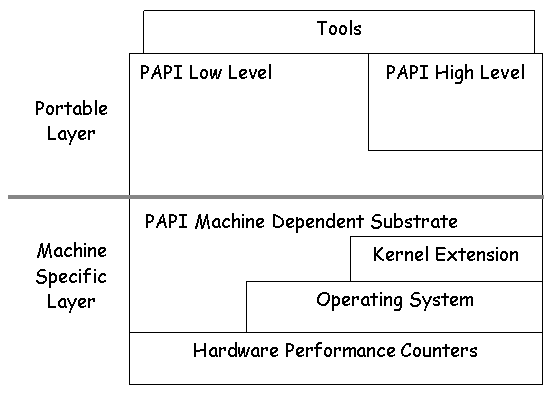
\includegraphics[width=12cm, height=8cm]{./images/papi}
\centering
\caption{Internal architecture of PAPI}
\label{fig:papi}
\end{figure}  

\par Above figure \ref{fig:papi} shows the internal architecture of PAPI. The architecture is divided into two parts, portable layer and machine specific layer. Portable layer has low level, high level and machine independent support functions. Whereas machine dependent layer consists of machine dependent functions and data structures. Layer also consists kernel extensions and operating system calls or assembly language to retrieve the data from counters of PMU. PAPI provides two interfaces, High level API and Low level API. High level API is easy to use and require less set-up but it has higher overhead and less flexibility. Considering that Low level API provides fine grained measurements, more control to interface and increase the functionality and efficiency. 

\par PAPI also provides command line interface event queries for existence of native or preset event to give more light about hardware supports specific events. Following code shows the PAPI API calls in code.  

\begin{lstlisting}
#include <papi.h>
#define NUM_EVENTS 2 

int main()
{
int Events[NUM_EVENTS] = {PAPI_TOT_INS, PAPI_TOT_CYC};
long_long values[NUM_EVENTS];
/* Start counting events */
if (PAPI_start_counters(Events, NUM_EVENTS) != PAPI_OK)
   handle_error(1); 
for (int i=0;i<1000:i++); 
if (PAPI_read_counters(values, NUM_EVENTS) != PAPI_OK)
   handle_error(1);
if (PAPI_stop_counters(values, NUM_EVENTS) != PAPI_OK)
   handle_error(1);
}
\end{lstlisting}

\par Following stats are showing the performance of Basicmath application from MiBench suite[]. Performance data is collected using PAPI API on Cortex A53 on single core that is core 2. 
\begin{lstlisting}
 $sudo ./runme_large.sh
 cycles:		1653593201,
 instructions:	1397640501,
 L2 cache miss:	2178,
 branches:	137950307,
 branch misses:	2668136
\end{lstlisting}

\subsection{Streamline Performance Analyzer}
Streamline Performance Analyzer is system-wide visualizer and profiler tool from ARM for ARMv7 and ARMv8 hardware targets. It generates the processor profile by reading the program counter at regular sample and collect the information about where processor spends its time. It collects the information of micro-architectural events from PMU of target hardware. Streamline gathers the performance data by communicating with software agent on target hardware. Streamline uses two communications agents, gator and barman. Gator is use for Linux targets whereas barman used for bare metal targets. 

\par In Streamline, best requisite set of hardware performance counters are used by default. But it is possible to change the configuration of hardware counters using Counter configurations dialog, which contains the list of available hardware performance counter for given specific target hardware. Streamline collects data in terms of samples and there are two modes of collecting samples in Streamline. One is fixed rate, where samples are collected in fixed intervals of time and this option is default in sampling method. Other method is Event-based sampling, where sampling is done on context switching or when an event occurs number of times.

\par Streamline provides Graphical User Interface (GUI). It shows captured data graphically. Streamline provides the functionality to capture data with counter configuration, start and stop of new captures of performance data. It provides live capture where in real time performance data is shown graphically in Streamline window for application being measured or profiled. It plots the counters in real time. After completion of the capture,capture information is shown in charts and details panel. Call paths in Streamline displays a hierarchy of functions, thread, processes. It also lists all functions in application called while capture. It also shows the core wise execution of thread and processes. Streamline also provide statistics line by line for source code. It also provides the string annotations and markers features which allows to add context to the information. Following image \ref{streamline} show the performance data collected for basicmath application from MiBench suite[] on Cortex A53 processor using Streamline performance analyzer. 

\begin{figure}[h!]
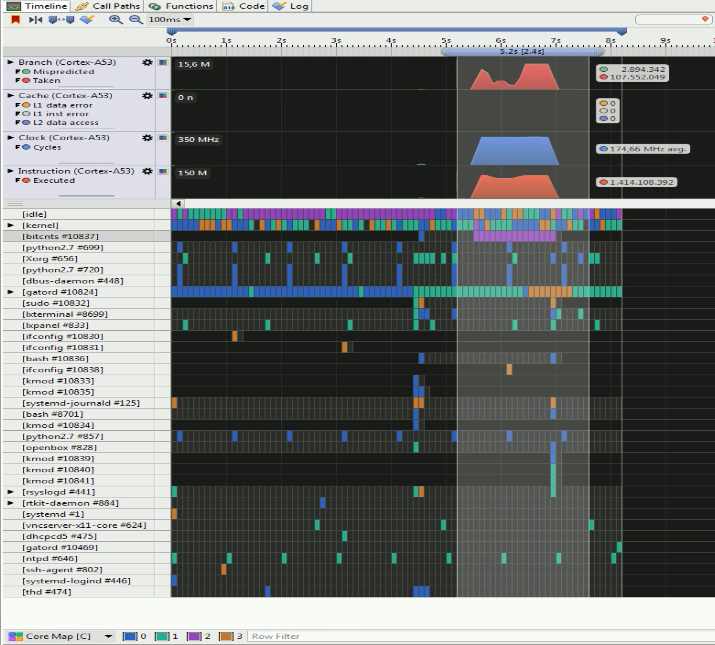
\includegraphics[width=16cm, height=12cm]{./images/streamline}
\centering
\caption{Timeline of basicmath application using Streamline Performance Analyzer}
\label{fig:streamline}
\end{figure} 

\section{Tools for Framework Development}
Apart from performance measurement tools, in this thesis we are also using tools which are freely available to use and create the framework for performance measurement. We are going to see LLVM compiler infrastructure project and Instruction Set Simulator(ISS) for create virtual simulation of hardware. 

\subsection{LLVM}
LLVM is collection of compiler and toolchain technologies used for development of front end and back end of compiler. Low level toolscahins like assemblers, debuggers, etc. LLVM started as a research project at University of Illinois. Initial motivation of LLVM was investigate dynamic compilation technique for static and dynamic programming languages[llvm.org]. LLVM is written in C++ language and it is designed for programs written in arbitrary programming language. Clang is LLVM native C/C++ compiler which provides more features than GCC and faster than GCC. Over last decade, LLVM is used as common infrastructure to implement runtime compiled languages, family of languages supported by GCC, Java, .NET, Python, Ruby, Scheme, etc. 

\par Traditional and popular design for compiler is divided into three major components, those components are the front end, the optimizer and the backend. The frontend component perform parsing of source code, checking the errors and represent the input code. The optimizer component try to improve the code by eliminating redundant computations and it is independent of language and target hardware architectures. The backend component converts the code into machine code compatible with target hardware architecture. One of the major implication of this design is that retargetability. If compiler uses common code representation for it's optimizer then backend can written for any target hardware architecture and frontend can be written for any source language. Which eliminate the wide number of compilers for each source language and for each hardware architecture. One of the successful implementation of this mode is GCC. It supports many frontends and backends and have wide community of contributors. 

\par  But there are limitations to this traditional approach. They are designed as monolithic applications for example GCC. Some pieces of libraries can not be reused. It has uncontrolling use of global variables, weakly enforced invariants, poorly-designed data structures, sprawling code base, and the use of macros that prevent the codebase from being compiled to support more than one front-end/target pair at a time. GCC suffers from layering problems and leaky abstractions: the back end walks front-end ASTs to generate debug info, the front ends generate back-end data structures, and the entire compiler depends on global data structures set up by the command line interface [chris lattner]. 

\par LLVM uses Intermediate Representation(IR) for code representation in compiler infrastructure. For any source code at frontend is converted into IR code and given to optimizer and output of the optimizer is also IR code which is faded to backend to create target machine code. You can see this behavior in following figure \ref{fig:llvm} of three phase structure of LLVM compiler. 

\begin{figure}[h!]
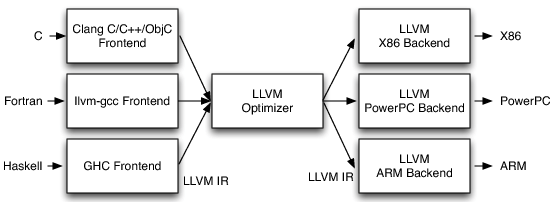
\includegraphics[width=12cm, height=6cm]{./images/llvm}
\centering
\caption{LLVM's three phase design}
\label{fig:llvm}
\end{figure}

LLVM IR is low-level Reduced Instruction Set Architecture(RISC) like virtual instruction set. We can see in this following example. 

\begin{lstlisting}
define i32 @add1(i32 %a, i32 %b) {
entry:
  %tmp1 = add i32 %a, %b
  ret i32 %tmp1
}

define i32 @add2(i32 %a, i32 %b) {
entry:
  %tmp1 = icmp eq i32 %a, 0
  br i1 %tmp1, label %done, label %recurse

recurse:
  %tmp2 = sub i32 %a, 1
  %tmp3 = add i32 %b, 1
  %tmp4 = call i32 @add2(i32 %tmp2, i32 %tmp3)
  ret i32 %tmp4

done:
  ret i32 %b
}
\end{lstlisting}

This is the LLVM IR for following C code. 

\begin{lstlisting}
unsigned add1(unsigned a, unsigned b) {
  return a+b;
}

unsigned add2(unsigned a, unsigned b) {
  if (a == 0) return b;
  return add2(a-1, b+1);
}
\end{lstlisting}

LLVM IR representation help to understand the code at machine level. LLVM also provide optimization at IR representation. LLVM is collection of libraries. LLVM also offers optimizations in terms of passes. LLVM passes is written in C++ class.  These passes traverse portion of program to either collect the information or transform the program. In this thesis we are going make use LLVM basic block pass to collect the performance data at basic block level. We will see it in detail in further chapters. LLVM also provide retargetablity for various source code languages and target architectures. It also provides capabiites by modular design such as when and where each phase of compiler runs, unit testing the optimizer and automatic test case reduction. 

\subsection{Instruction Set Simulator}
Instruction Ste Simulators(ISS) is simulation model and mostly coded into high level programming languages. This simulation models reflects the behavior of actual microprocessor/microcontroller. This simulation models can mimic various hardware architectures. ISS mimics the behavior by reading the assembly instructions and maintaining the processor registers. ISS are widely used for simulating the machine code of another hardware to check compatibility, monitoring and testing of machine code, testing and debugging of machine code, and to improve the performance. ISS are important in early embedded product release in market. It can help to simulate target hardware if it is not available in market or in prototype phase of development. Disadvantage of ISS is that they costly and oftenely they are slow. 

\section{Basic Learning Techniques}
It is possible to get mathematical relationship between input and respective output by observing the behavior. Mathematical statement or equation is formed using this one to one, one to many, many to one or many to many. Mathematical relationship can be formed by creating with support the dataset of this relationship. The dataset contains the history of wide range data of input and output. This analysis of of input output model helps to create statistical model that can be useful predict output for new every input using learned mathematical model and accurate dataset. 

\par This relationship between input and output is learned using Machine Learning. Machine learning techniques allows to form this relationship and create dataset to predict the result for every new input. This is done by without any explicit programming. Only important thing is create dataset of input and output that helps to understand the behavior of relationship between them. And mathematical model can be created to learned this relationship and used to predict the output. There basically three main machine learning techniques are available,they are, supervised learning, unsupervised learning and regression learning. Again in these three main learning techniques many sub-techniques are available. Obtained dataset in machine learning filed is called as training data. Which helps to understand the behavior. Machine learning technique is any application is depending upon relationship between input and output and use case. In some cases relationship is linear or in some cases data is in number of chunks.

\subsection{Regression}
Regression is most popular technique in the field of machine learning, in which linear regression and logistic regression are most widely used and known to data analytics.  There are also regression techniques are available. Regression is popular statistical techniques use for application of predictive modeling. In regression technique, relationship model is formed in between dependent variable and independent variable. These variable can be one or many. For example in annual sale prediction, sales is dependent variable whichis going to predicted whereas factors affecting the sales are independent variables, these can be one or many. 

\par In linear regression techniques, dependent variable is continuous in nature with respect to independent variable. And relationship between these variable is assumed to be linear in nature. Logistic regression method is used for classification. Classification can binary or multi-class classification. There are also different techniques such as lasso regression, ridge regression, 
and many more techniques are available. These techniques are depend upon application and analysis of the data. We will see in more detail in upcoming chapters.








  % Load Data from File intro.tex
\chapter{Basics}
% ------------------------------------------------------------------------------
% Chapter 3 : Setup steps and Basic Usage Insight
% ------------------------------------------------------------------------------
\setlength{\parindent}{4em}
\setlength{\parskip}{1em}

In this section we will go through basics like performance measurement concept, tools to measure performance, LLVM, instruction set simulator(ISS) and basic learning techniques to understand the thesis. Performance of software on embedded hardware is essential in embedded product development. The measure question is how to measure performance of software on hardware. Here software maybe an application or operating system. Performance of application or operating system can be  analyzed and improved using performance monitoring features provided by embedded hardware. Now every modern hardware processor has Performance Monitoring Unit(PMU) on chip. PMU is on-chip hardware device that monitors the micro-architectural events. Events like cache hits, cache miss, cycles etc. Data collected from PMU can be use to observe the behavior of application or operating system on hardware processor. This collected data can be use to improve the performance. 

\par Performance monitoring events can be categorized in two types, one is hardware events and second is software events. Hardware events contain the events related to hardware like cycles, instructions, cache miss, cache hit etc. Where software events are related to software like page fault, segmentation fault, context switch etc. Performance monitoring hardware consists two components, performance event select registers and event counters. Performance event select registers are configuration registers to control what events to be monitored and how to monitor. Event counters registers, those count the number of events based on event select registers configuration. Also there are two approaches for performance monitoring, one is counting and other is event based sampling. Following figure \ref{fig:pmu} shows the block diagram of PMU in ARM Cortex A53 processor. 

\begin{figure}[h!]
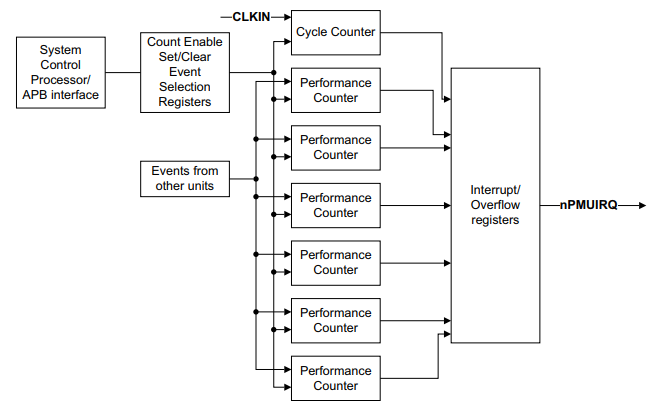
\includegraphics[width=14cm, height=10cm]{./images/pmu}
\centering
\caption{Block diagram of PMU in ARM Cortex A53 processor}
\label{fig:pmu}
\end{figure}

\section{Tools for Performance Measurement}
To evaluate the performance of software on hardware, variety of tools are available. These tools provide high level interface and analysis capabilities for performance monitoring hardware. The Performance Application Programming Interface (PAPI) tool suite [papi link] provides a common interface to performance monitoring hardware for many different processors like Alpha, ARM, MIPS, Pentium, PowerPC and etc. VTune Performance Analyzer [link for it] from Intel support performance monitoring on Intel's processor. PERF is performance analyzing tool in Linux, available from Linux kernel version 2.6.31 [link for perf]. OProfile[link for OProfile] is system-wide  statistical profiling tools for Linux to measure the performance of underlying hardware processor. ARM's Streamline Performance Analyzer provide in depth look of software performance on ARM processors. In this thesis, we are going to see tools like PAPI, PERF and Streamline Performance analyzer to evaluate the performance of software. In this thesis, we are focusing on hardware events and the performance data provided by these performance measurement tools measured on Raspberry Pi 3B board, which includes ARM Cortex A53 processor.

\subsection{PERF}
PERF is performance analyzing tool in Linux operating system and it is available from version 2.6+ of Linux kernel. PERF can accessed by userspace controlling utility, named 'perf'. PERF command line interface on Linux provides number of subcommands. PERF provides statictical data performance data of Linux kernel and user application. PERF supports hardware performance counters, software performance counters and tracepoints. PERF is based on 'perf\_events' interface. 

\par PERF Linux tool supports wide majority of events to provide the performance data. This tool can measure events from different sources using kernel interface. One source of events are kernel counters and these events are called software events like context switches, page-fault, alignment fault, emulation fault and etc. Another source of events is processor itself. PERF reads the events from hardware performance counter of PMU of processor. PERF provides the list micro-architectural events supported by it such as number of cycles, L1 cache miss, total instructions, branch mispredicted and many more.  Finally, the tracepoint events which are provided by kernel through 'ftrace' infrastructure.

\par One of the main feature of the PERF is that it allowed to select the specific core/s of processor using processor-wide mode. The performance data of specific core/s  can be collected for given application or operating system. Which had very significance in this thesis. It also creates the report of the collected sample data in file called 'perf.data'.It also possible with PERF to go more in granularity of instruction level with 'perf annotate'. 	PERF also provide the live analysis like Linux top command with processor wide feature. it is possible to measure the performance of application in userspace as well as kernel space. 

\par PERF provides subcommands on command line interface such as 'stat, record, report', etc. It is possible to get the list of software and hardware events supported by PERF using 'list' command for running embedded hardware processor. Following is the PERF usage on Raspberry Pi 3B board with Raspbian, Linux based operating system and we are measuring the performance of basicmath application from Mibench suite[] for single core i.e. second core of Cortex A53..


\begin{lstlisting}
$ sudo perf_3.16 state -e cycles,instructions,cache-misses,
 branches,branch-misses -C 2 ./runme_large.sh

# started on Wed Apr  4 14:02:59 2018 

Performance counter stats for 'CPU(s) 2':     
1,654,827,425      			cycles                        
1,397,787,969      			instructions              #    0.84  insns per cycle                    
3,528     	 				cache-misses                                                       
94,047,959     	 			branches                                                             
2,669,120    	 			branch-misses          #    2.84% of all branches              
2.445278109 seconds time elapsed
\end{lstlisting}

\subsection{PAPI}
PAPI is abbreviation for Performance Application Programming Interface. PAPI project is developed at University of Tennessee's Innnovative Computing Laboratory in Computer Science Department. This project was created to design, standardize, and implement a portable and efficient Application Programming Interface (API) to access the hardware performance counters found on most modern microprocessors[papi user guide]. PAPI provides an API to read hardware performance counter values for application running on processor. This data can be use to improve the performance of application or code. Similar kinds of APIs are available but PAPI provides stable API, documentation and upgrade it with features and different platforms. 

\par PAPI provides solid base for cross-platform tools. It provides standardize API. It is easy to use and freely available. It provides consistent interface and methodology to tool designers as well as application engineers to collect data from performance counters of PMU.  It provides near real time performance data between application and processor events. PAPI provides operating system independent access to hardware performance counters. 

\begin{figure}[h!]
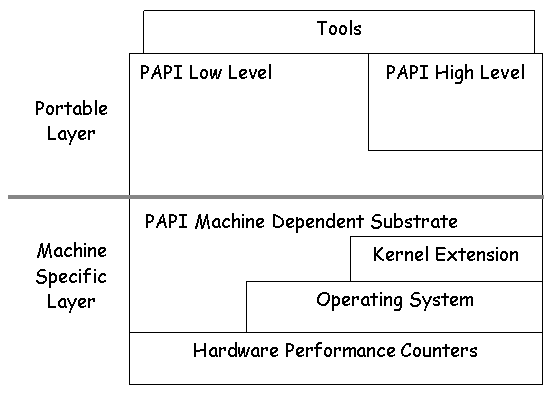
\includegraphics[width=12cm, height=8cm]{./images/papi}
\centering
\caption{Internal architecture of PAPI}
\label{fig:papi}
\end{figure}  

\par Above figure \ref{fig:papi} shows the internal architecture of PAPI. The architecture is divided into two parts, portable layer and machine specific layer. Portable layer has low level, high level and machine independent support functions. Whereas machine dependent layer consists of machine dependent functions and data structures. Layer also consists kernel extensions and operating system calls or assembly language to retrieve the data from counters of PMU. PAPI provides two interfaces, High level API and Low level API. High level API is easy to use and require less set-up but it has higher overhead and less flexibility. Considering that Low level API provides fine grained measurements, more control to interface and increase the functionality and efficiency. 

\par PAPI also provides command line interface event queries for existence of native or preset event to give more light about hardware supports specific events. Following code shows the PAPI API calls in code.  

\begin{lstlisting}
#include <papi.h>
#define NUM_EVENTS 2 

int main()
{
int Events[NUM_EVENTS] = {PAPI_TOT_INS, PAPI_TOT_CYC};
long_long values[NUM_EVENTS];
/* Start counting events */
if (PAPI_start_counters(Events, NUM_EVENTS) != PAPI_OK)
   handle_error(1); 
for (int i=0;i<1000:i++); 
if (PAPI_read_counters(values, NUM_EVENTS) != PAPI_OK)
   handle_error(1);
if (PAPI_stop_counters(values, NUM_EVENTS) != PAPI_OK)
   handle_error(1);
}
\end{lstlisting}

\par Following stats are showing the performance of Basicmath application from MiBench suite[]. Performance data is collected using PAPI API on Cortex A53 on single core that is core 2. 
\begin{lstlisting}
 $sudo ./runme_large.sh
 cycles:		1653593201,
 instructions:	1397640501,
 L2 cache miss:	2178,
 branches:	137950307,
 branch misses:	2668136
\end{lstlisting}

\subsection{Streamline Performance Analyzer}
Streamline Performance Analyzer is system-wide visualizer and profiler tool from ARM for ARMv7 and ARMv8 hardware targets. It generates the processor profile by reading the program counter at regular sample and collect the information about where processor spends its time. It collects the information of micro-architectural events from PMU of target hardware. Streamline gathers the performance data by communicating with software agent on target hardware. Streamline uses two communications agents, gator and barman. Gator is use for Linux targets whereas barman used for bare metal targets. 

\par In Streamline, best requisite set of hardware performance counters are used by default. But it is possible to change the configuration of hardware counters using Counter configurations dialog, which contains the list of available hardware performance counter for given specific target hardware. Streamline collects data in terms of samples and there are two modes of collecting samples in Streamline. One is fixed rate, where samples are collected in fixed intervals of time and this option is default in sampling method. Other method is Event-based sampling, where sampling is done on context switching or when an event occurs number of times.

\par Streamline provides Graphical User Interface (GUI). It shows captured data graphically. Streamline provides the functionality to capture data with counter configuration, start and stop of new captures of performance data. It provides live capture where in real time performance data is shown graphically in Streamline window for application being measured or profiled. It plots the counters in real time. After completion of the capture,capture information is shown in charts and details panel. Call paths in Streamline displays a hierarchy of functions, thread, processes. It also lists all functions in application called while capture. It also shows the core wise execution of thread and processes. Streamline also provide statistics line by line for source code. It also provides the string annotations and markers features which allows to add context to the information. Following image \ref{streamline} show the performance data collected for basicmath application from MiBench suite[] on Cortex A53 processor using Streamline performance analyzer. 

\begin{figure}[h!]
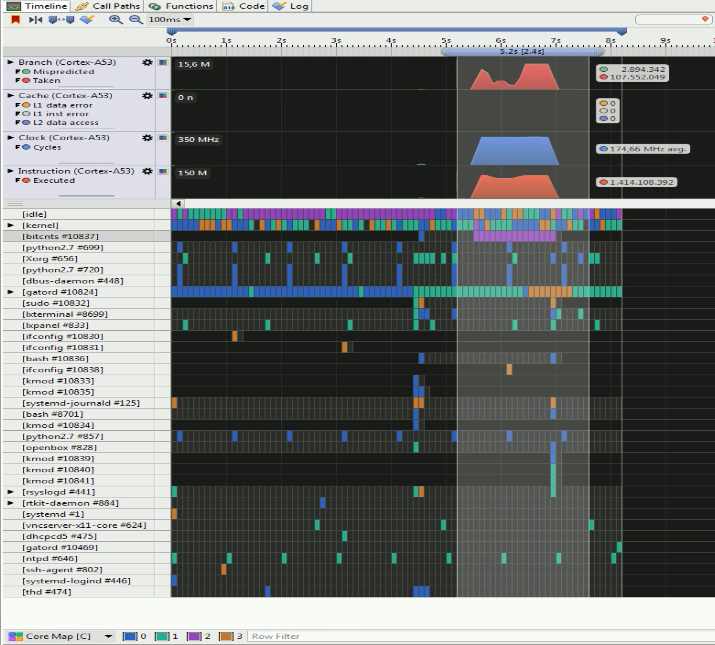
\includegraphics[width=16cm, height=12cm]{./images/streamline}
\centering
\caption{Timeline of basicmath application using Streamline Performance Analyzer}
\label{fig:streamline}
\end{figure} 

\section{Tools for Framework Development}
Apart from performance measurement tools, in this thesis we are also using tools which are freely available to use and create the framework for performance measurement. We are going to see LLVM compiler infrastructure project and Instruction Set Simulator(ISS) for create virtual simulation of hardware. 

\subsection{LLVM}
LLVM is collection of compiler and toolchain technologies used for development of front end and back end of compiler. Low level toolscahins like assemblers, debuggers, etc. LLVM started as a research project at University of Illinois. Initial motivation of LLVM was investigate dynamic compilation technique for static and dynamic programming languages[llvm.org]. LLVM is written in C++ language and it is designed for programs written in arbitrary programming language. Clang is LLVM native C/C++ compiler which provides more features than GCC and faster than GCC. Over last decade, LLVM is used as common infrastructure to implement runtime compiled languages, family of languages supported by GCC, Java, .NET, Python, Ruby, Scheme, etc. 

\par Traditional and popular design for compiler is divided into three major components, those components are the front end, the optimizer and the backend. The frontend component perform parsing of source code, checking the errors and represent the input code. The optimizer component try to improve the code by eliminating redundant computations and it is independent of language and target hardware architectures. The backend component converts the code into machine code compatible with target hardware architecture. One of the major implication of this design is that retargetability. If compiler uses common code representation for it's optimizer then backend can written for any target hardware architecture and frontend can be written for any source language. Which eliminate the wide number of compilers for each source language and for each hardware architecture. One of the successful implementation of this mode is GCC. It supports many frontends and backends and have wide community of contributors. 

\par  But there are limitations to this traditional approach. They are designed as monolithic applications for example GCC. Some pieces of libraries can not be reused. It has uncontrolling use of global variables, weakly enforced invariants, poorly-designed data structures, sprawling code base, and the use of macros that prevent the codebase from being compiled to support more than one front-end/target pair at a time. GCC suffers from layering problems and leaky abstractions: the back end walks front-end ASTs to generate debug info, the front ends generate back-end data structures, and the entire compiler depends on global data structures set up by the command line interface [chris lattner]. 

\par LLVM uses Intermediate Representation(IR) for code representation in compiler infrastructure. For any source code at frontend is converted into IR code and given to optimizer and output of the optimizer is also IR code which is faded to backend to create target machine code. You can see this behavior in following figure \ref{fig:llvm} of three phase structure of LLVM compiler. 

\begin{figure}[h!]
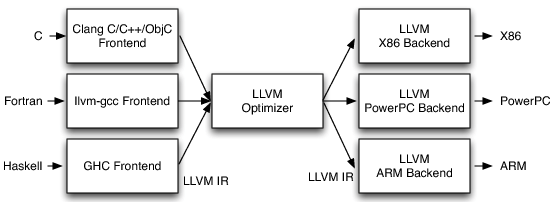
\includegraphics[width=12cm, height=6cm]{./images/llvm}
\centering
\caption{LLVM's three phase design}
\label{fig:llvm}
\end{figure}

LLVM IR is low-level Reduced Instruction Set Architecture(RISC) like virtual instruction set. We can see in this following example. 

\begin{lstlisting}
define i32 @add1(i32 %a, i32 %b) {
entry:
  %tmp1 = add i32 %a, %b
  ret i32 %tmp1
}

define i32 @add2(i32 %a, i32 %b) {
entry:
  %tmp1 = icmp eq i32 %a, 0
  br i1 %tmp1, label %done, label %recurse

recurse:
  %tmp2 = sub i32 %a, 1
  %tmp3 = add i32 %b, 1
  %tmp4 = call i32 @add2(i32 %tmp2, i32 %tmp3)
  ret i32 %tmp4

done:
  ret i32 %b
}
\end{lstlisting}

This is the LLVM IR for following C code. 

\begin{lstlisting}
unsigned add1(unsigned a, unsigned b) {
  return a+b;
}

unsigned add2(unsigned a, unsigned b) {
  if (a == 0) return b;
  return add2(a-1, b+1);
}
\end{lstlisting}

LLVM IR representation help to understand the code at machine level. LLVM also provide optimization at IR representation. LLVM is collection of libraries. LLVM also offers optimizations in terms of passes. LLVM passes is written in C++ class.  These passes traverse portion of program to either collect the information or transform the program. In this thesis we are going make use LLVM basic block pass to collect the performance data at basic block level. We will see it in detail in further chapters. LLVM also provide retargetablity for various source code languages and target architectures. It also provides capabiites by modular design such as when and where each phase of compiler runs, unit testing the optimizer and automatic test case reduction. 

\subsection{Instruction Set Simulator}
Instruction Ste Simulators(ISS) is simulation model and mostly coded into high level programming languages. This simulation models reflects the behavior of actual microprocessor/microcontroller. This simulation models can mimic various hardware architectures. ISS mimics the behavior by reading the assembly instructions and maintaining the processor registers. ISS are widely used for simulating the machine code of another hardware to check compatibility, monitoring and testing of machine code, testing and debugging of machine code, and to improve the performance. ISS are important in early embedded product release in market. It can help to simulate target hardware if it is not available in market or in prototype phase of development. Disadvantage of ISS is that they costly and oftenely they are slow. 

\section{Basic Learning Techniques}
It is possible to get mathematical relationship between input and respective output by observing the behavior. Mathematical statement or equation is formed using this one to one, one to many, many to one or many to many. Mathematical relationship can be formed by creating with support the dataset of this relationship. The dataset contains the history of wide range data of input and output. This analysis of of input output model helps to create statistical model that can be useful predict output for new every input using learned mathematical model and accurate dataset. 

\par This relationship between input and output is learned using Machine Learning. Machine learning techniques allows to form this relationship and create dataset to predict the result for every new input. This is done by without any explicit programming. Only important thing is create dataset of input and output that helps to understand the behavior of relationship between them. And mathematical model can be created to learned this relationship and used to predict the output. There basically three main machine learning techniques are available,they are, supervised learning, unsupervised learning and regression learning. Again in these three main learning techniques many sub-techniques are available. Obtained dataset in machine learning filed is called as training data. Which helps to understand the behavior. Machine learning technique is any application is depending upon relationship between input and output and use case. In some cases relationship is linear or in some cases data is in number of chunks.

\subsection{Regression}
Regression is most popular technique in the field of machine learning, in which linear regression and logistic regression are most widely used and known to data analytics.  There are also regression techniques are available. Regression is popular statistical techniques use for application of predictive modeling. In regression technique, relationship model is formed in between dependent variable and independent variable. These variable can be one or many. For example in annual sale prediction, sales is dependent variable whichis going to predicted whereas factors affecting the sales are independent variables, these can be one or many. 

\par In linear regression techniques, dependent variable is continuous in nature with respect to independent variable. And relationship between these variable is assumed to be linear in nature. Logistic regression method is used for classification. Classification can binary or multi-class classification. There are also different techniques such as lasso regression, ridge regression, 
and many more techniques are available. These techniques are depend upon application and analysis of the data. We will see in more detail in upcoming chapters.








  % Load Data from File intro.tex
%------------------------------------------------------------------------------
% Chapter 4 : Design and Implementation Storyboards
%------------------------------------------------------------------------------
\chapter{Design and Implementation Storyboards}
% ------------------------------------------------------------------------------
% Chapter 4 : Analysis of Missing Features and Concepts
% ------------------------------------------------------------------------------
\setlength{\parindent}{4em}
\setlength{\parskip}{1em}

\section{Analysis}
Objective of this thesis is to estimate the performance of software or application on embedded hardware platform. And  performance aspect is total number of cycles. There different methods and techniques are available to evaluate the performance of software on given hardware platform. Techniques such as simlution techniques, WCET analysis, statistical and analyticl models, performance measurement tools and many more. Current state of the art tells us different methodology to estimate or calculate or predict the performance of software on hardware platform. Performance is measured on single-core or multi-core hardware platforms. But every technique or methodology has it's advantages and disadvantages which provide an opportunity to create new methodology or improve the existing technique with resolving drawbacks. With state of the art, in this thesis we ware going to see current disadvantages and missing features in state of the art and how can be these disadvantages are overcome and missing features can be added. 

\subsection{Analysis of Simulators}
\par Simulator is one the widely used to model hardware platform into virtual software platform. Where it provide an opportunity with market demand unavailable hardware can be implemented on simulators. Some hardware platforms are in developing stages or only have prototypes of it. In such cases it is difficult to finish embedded product within timeline. In above state of the art, Instruction Set Simulators(ISS) is used for Learning-based analytical cross-platform performance prediction[ieee1]. ISS simulates the Instruction Set Architecture(ISA). In given approach Target platform is simulated using gem5 simulator. In simulator, authors created virtual model of ARM processor and total number of cycles are extracted from it. Also in method[] mentioned for uniprocessor and multiprocessor performance evaluation of software, simulators are used. 

\par Cycle accurate simulators provide accurate cycles by simulation microarchitecture cycle by cycle basis. As we saw from ARM two cycle accurate simulators are available with trade of simulation speed and abstraction level. Following are the advantage and disadvantages of simulators are discussed with respect to state of the art and thesis agenda.

\subsubsection{Advantages}
\begin{itemize}
   \item Create exact simulation model of hardware platform. 
   \item Suitable when hardware platform is unavailable of in prototype phase.
   \item Full system models can also run operating systems on simulators.
\end{itemize}

\subsubsection{Disadvantages}
\begin{itemize}
   \item Majority of Simulators available in market are slowas compared to native hardware platform.
   \item Major drawback is cost. Simulators are more costly.
   \item There are dependencies while installing simulators on host platforms. 
\end{itemize}

\subsection{Analysis of Performance Measurement Tools}
Performance measurement tools extract the information from PMU of hardware platform by reading hardware performance counters. Hardware performance counters contains the information about microarchitecture events like cache misses, cache hits, etc. To evaluate the performance of software or application on given hardware platform, microarchitecture event data help. In given state of the art, PAPI is only performance analysis tools is used in methods discussed by Gerstlauer[iee1,ieee2]. But there are many performance analyzer tools are available in market such as PERF, ARM streamline performance analyzer, Oprofile and many more. These tools are not explored in given approaches. Whereas on target platforms, cycles are calculated using cycle accurate simulators.

\subsubsection{Advantages}
\begin{itemize}
   \item Easy to understand the performance of software on given hardware.
   \item Some tools provide graphical user interface(GUI) and more features to analyze the data like ARM Streamline. 
   \item Some tools are free because of open source licenses like PAPI, PERF, OProfile.
\end{itemize}

\subsubsection{Disadvantages}
\begin{itemize}
   \item GUI tools are expensive.
   \item Set-up of measurement for GUI tools is complicated. 
   \item In some tools, all microarchitectural events are not available.
\end{itemize}


\subsection{Analysis of performance data collection on number of core}
As we know modern day processors have multi-core in SoC. And performance evaluation on multi-core processor is hard task. In state of the art analytical approaches, all data is collected on single core using performance measurement tools where in approach of uniprocessor and multiprocessor,performance data is collected on simulators not on native harwdare platforms. Also uniprocessor performance data is used to evaluate the performance of the software on dual-core and quad-core processors.

\subsection{Analysis of grouping of hardware performance counters}
Performance measurement tools read the hardware performance counter data and provide to user. Every processor has different number of hardware performance counters are available in it. To evaluate the performance of software, some performance analyzer tools provides access to limited number of hardware performance counter out of number of available hardware performance counters. So for same software, measurements need to be taken again because of limited availability at single time. Whereas PERF provides access to all hardware performance counters but the using sampling method and numbers are not accurate. This is measure drawback of performance measurement tools. In such scenarios the either only effective hardware performance counters considered or grouping of the hardware performance counter is performed and repeated measurements are taken. 

\subsection{Analysis of Data Analysis Techniques}
In analytical model approaches, all performance data is collected by executing number of softwares or application on host and target hardwares. This data is purposed for training data or for test data. If it is purposed for training data then analysis of data is important. Analysis of data collected can help to understand the data and behavior of software on given platforms. Data analysis technique application on large collected data helps to choose the learning algorithms. 


\section{Contribution to Thesis}
In previous chapter, we have seen the advantage and disadvantages of tools and techniques used in state of the art methodology to estimate the performance of software on hardware platform. All these drawbacks can be eliminated and all advantages can use to make single approach. That single approach is able to estimate the performance of software at phase level where phase size defined by user, on native hardware platform, on single-core and dual-core, with technique of data analysis involved and learning algorithms to estimate the performance. 

\par In this thesis, software performance measurement tools are explored and chosen accordingly. As we saw in previous chapter, that there wide variety of software performance tools available in market. Some of them are open source license and some of them are paid. These measurement tools provide data regarding performance of software to user which helps to understand the performance behavior of software on given hardware platform. With help of this statistics, performance of software can be improved. Measurement tool like ARM Stream line provides the visualization of live performance measurement, which help to understand the flow of software execution. Also Linux tools like PERF, which is open source license provide the data for each hardware performance counter and helps to automate the scripts in Linux environment. PAPI provides low level and level API calls to measure the performance of software. Exploration of the all tools performed in this thesis and best suited tool for application is used to collect the data at phase level of software.

\par As we know the performance of embedded processor and processor used in modern personal or office computer is quite different. ARM processors are most commonly used in embedded applications where as Intel processors are used in computers. These processors have different characteristics. Such as, ARM processor has fewer and simple instructions as compared to Intel so they have different processing powers. Power consumption is also crucial between thes two processor categories. Embedded processors consume less power as compared to computer processors. Also there is differences between software in these processor. Operating systems is used for both platforms is application specific and performance specific. Also use of the processor depend upon the application and cost of the product. In this thesis, our focus is on embedded processor and estimating the performance of software or application on it.

\par In previous chapters, we discussed about the grouping of the hardware performance counters. Performance measurement tools access the hardware performance counters, which monitors the microarchitectural events. In this thesis we are going to see grouping of the counters. Number of hardware performance counters vary from processor to processors. It is not possible for performance measurement tools to access all hardware performance counters at same time. For example PAPI can access only six hardware performance counter at single time. In such cases, grouping of hardware performance counter is important. It help to understand the impact of each hardware performance counter on other counters and according to that different combinations can be implemented and best groups can be selected to observe the performance. Grouping of hardware performance counter plays measure roles. 

\par In this thesis work, we are going to use learning model approach to predict the performance. In machine learning, ill-formed and insufficient data can affect the learning model. A good training set data is important to train the machine learning algorithm. Data collected for training data can be big. It is important to understand the behavior of collected data. In this case data analysis techniques come handy. These techniques provide visualization of data collected and help to analyze the data. For example correlation coefficient, principal component analysis and many more data analysis techniques are used. 

\par Also current thesis work focuses on performance estimation on dual-core processors. As we saw in current state of the art, performance is evaluated on single core using learning model. Where as uniprocessor and multiprocessor approach estimated the performance on dual-core and quad-core but using simulation on Intel processor. And this thesis is focused on software performance prediction on dual-core of embedded hardware platform.  % Load Data from File intro.tex
%------------------------------------------------------------------------------
% Chapter 5 : Performance Measurements Tests
%------------------------------------------------------------------------------
\chapter{Safety Competency}
% ------------------------------------------------------------------------------
% Chapter 5 : Concept Description
% ------------------------------------------------------------------------------
\setlength{\parindent}{4em}
\setlength{\parskip}{1em}

This thesis work emphasis on analytical model technique to predict the performance on embedded hardware. This analytical model or statistical model contains large dataset of performance, collected from hardware platform using performance measurement tool at each phase level of software. 

\par Due to unavailability of hardware platform, it is difficult for software engineers to estimate the performance of developing software. Some time hardware may not be yet developed or it may be prototype phase. Without performance evaluation of software, optimization is not possible and product release get prolonged. In this thesis work total number of cycles is performance aspect for software. In such scenario, cycle accurate simulators can be used but one of the main disadvantage is that they are too slow and costly. For higher speed, fast cycle models are available but performance is measured at abstraction level and they are costly. There is no tools, framework or methodology available to which can provide speed higher than cycle accurate models and less abstraction level than fast cycle models. This criteria can be implemented using machine learning technique, that can provide accurate results with less abstraction. 

\par In this thesis work Raspberry Pi 3B[link] is used as host and target platform. Basic ideology is that, performance of software can be predicted by for same SoC without physical need of it. Software or application who's performance to be evaluated is executed on Raspberry and learning algorithm predicts the total number of cycles for it. 

\par Performance data for number of programs is collected by executing them on host platform. These data is collected at each phase of software. Each phase of software can be defined as number of basic blocks it contains. Size of phase depends on the number of basic blocks. This of each phase for software can be varied by user. This provides more fined granularity to understand the behavior of software at each phase while executing on hardware platform. For example granularity of 500 is defined by user it means each phase has 500 basic blocks and performance is measured for each phase of software. Basic block in software is line of codes which has straight sequence of execution without branching except it has single entry and single exit. Number of programs executed with different granularity level provide wide performance datasets. 

\par Main challenge is to collect the performance data at each phase and to collect the data we need performance measurement tool. Tool which is flexible to collect data at different user defined granularity level. But major challenge is how to divide the software in different phases. Tool chain is needed to convert the software in basic blocks, combine basic blocks at granularity defined by user and then measure performance at built phase. In this thesis we will see the framework which divides the software in number of basic block and combine them into user defined granularity and supports to measure performance data at phase level. 

\par Before dividing the software in different phases, selection of performance measurement tools is important aspect. As we discussed in previous chapters that there are many tools available such as PAPI, PERF, OProfile, ARM Streamline,etc. But while selecting tools accuracy, speed, flexibility, portability, and cost all these factors need be considered. Performance data showed by tools must be accurate. It provides the results as fast as possible. It should be flexible for application such as collecting data at phase level of software. It can be easily ported to other operating systems and hardware platforms. And main important factor is cost. Whether it is paid or free license. 

\par PMU of processor monitors the microarchitectural events. These microarchitectural events are read by performance measurement tools. In Raspberry Pi 3B, only 14 hardware performance counters are available. One of the drawback of accessing the hardware performance counters from PMU is limited counters used at a time. Tools like PAPI, PERF and Streamline can measure 6 hardware counters at a time. That mean to read other hardware counter values the software need to executed for at least three times to get reading for all 14 performance counters. In 14 hardware counters total cycle counter is also included. So to observe and understand the impact of each counter on cycle grouping of counters is needed to be done. So similar software is execute at least three times that means for during every execution background environment needs to be kept similar to avoid disturbances. 

\par This thesis focuses on performance evaluation on dual-core of processor. Methodology  or techniques used to collect the performance data on single core are different than dual-core processor. In single core mode, interrupts can be disabled and measurement process is easy by making single core isolated from other operating system and scheduler processes. Whereas in dual-core mode, collection is of performance data is hard. Task migration is one the measure issue while performance measurement on dual-core. Scheduler can migrate task between cores. Same time resource utilization, interrupts and many parameters affect the measurement process. In this thesis we proposes, two modes to measure performance data on dual-core, one is full load and another is no load. During one of the active mode performance data is collected on dual core and performance also predicted in same mode. 

\par Data analysis performs measure role in prediction using learning methods. Backbone of machine learning algorithms is training data. This training data must not be ill to give to learning algorithm. In this thesis work, large number of sample programs are executed on host platform in single core mode, dual-core no load mode and dual-core full load to collect performance data on it at basic block level. Due to data collected at basic block level, produced data is large and understand the data whether is wrong or not data analysis techniques need to be applied to collected dataset. Data analysis techniques allows to understand the data and behavor of it. It also helps to understand the relation between dependable and independable variables and corelation in between them with help of correlation coefficient technique of data analysis. Also data is collected in 13 dimensions in this thesis to analyze and visualize the 13 dimensional data is challenge. With help of Principal Component Analysis(PCA), it is possible to compress the data into 2 dimensions and perform visualization. All this techniques are mentioned in upcoming chapters. 



  % Load Data from File intro.tex
%------------------------------------------------------------------------------
% Chapter 6 : Functional Safety and Security
%------------------------------------------------------------------------------
\chapter{Performance Evaluation}
% ------------------------------------------------------------------------------
% Chapter 6 : Design and Implementation Storyboard
% ------------------------------------------------------------------------------
\setlength{\parindent}{4em}
\setlength{\parskip}{1em}

In this chapter, we are going to see scientific work carried out during this thesis. Implementation of this thesis is divided into two parts, training phase and prediction phase. In implementation, host and target platform is same that is Raspberry Pi 3B. It is referred as host platform in training framework and target platform in prediction framework. We will cover all technical details and methods used for each block in these frameworks.

\par First, we will look for the training phase. In training phase, an application is  feed to LLVM and then using LLVM and measurement tools, performance is measured at each phase on host platform. Same process is applied for wide number of application program written in programming language C/C++ to collect the training data. Following diagram \ref{fig:training} illustrate the training phase framework to collect the database. In further every component of framework is discussed in detail.

\begin{figure}[h!]
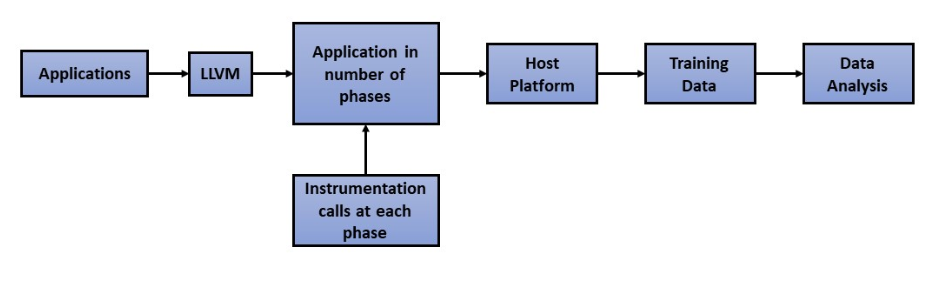
\includegraphics[width=14cm, height=5cm]{./images/training}
\centering
\caption{Training phase framework}
\label{fig:training}
\end{figure}

\section{Hardware platform}
In this thesis work, performance measurement for wide number of software applications are performed on Raspberry Pi 3B. Broadcom chip BCM2837 is used as SoC in Raspberry Pi 3B. This SoC uses ARM Cortex A53 quad core processor with 1 Giga Bytes of memory. It works on 1.2 GHz frequency. It supports MicroSD card for operating system and storing the data. Operating system used during this on Raspberry board was Raspbian Jessie which is open source license.

\par Processor on SoC of Raspberry is ARM Cortex A53. It is high efficiency processor for applications such automotive, mobile, DTV, networking, storage, aerospace and many more. It is based on Armv8-A architecture. It is quad core with Symmetrical Multiprocessing(SMP) within a single processor cluster, and multiple coherent SMP processor clusters through AMBA 4 technology[arm link a53]. Cortex A53 supports AARCH32 as well as AARCH64 instruction set architecture. It has full backward compatibility with Armv7 and it has 64 bit support. Raspbian Jessie is 32 bit OS and it was primary operating system during the thesis work. As it is 32 bit operating system, Cortex A53 was running on backward compatibility on Armv7 32 bit mode with AARCH32 ISA. It was not possible to use 64 bit mode with AARCH64 ISA. Following diagram \ref{fig:a53} from ARM[] illustrate the Cortex A53.

\begin{figure}[h!]
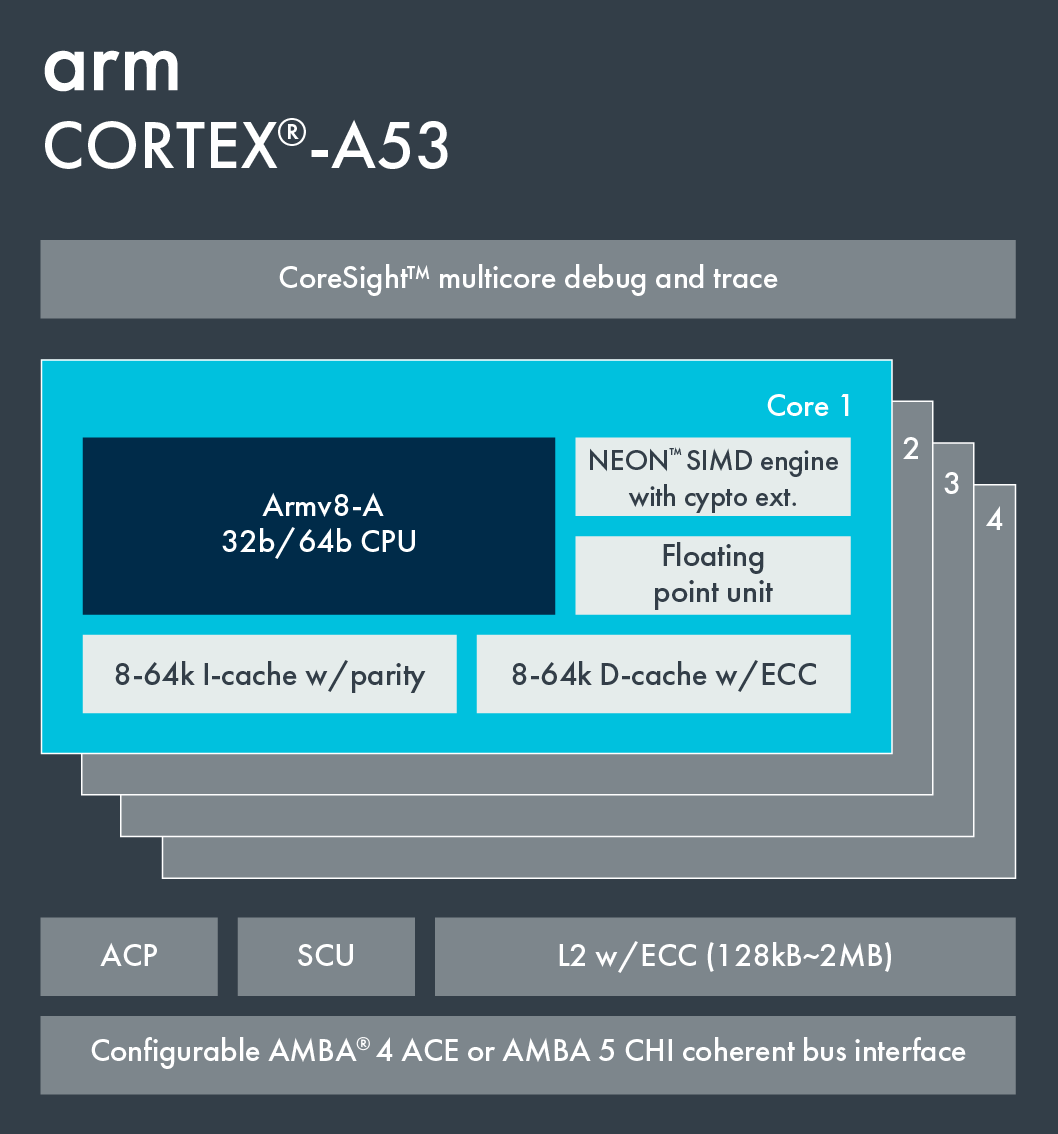
\includegraphics[width=8cm, height=12cm]{./images/A53}
\centering
\caption{Cortex A53[]}
\label{fig:a53}
\end{figure}

\par Cortex A53 has two level of cache hierarchy. Each core has level1 individual cache of 32kB. Level2 cache is unified for all cores with size of 512kB. As Raspberry was running on AARCH32 ISA, it was using AARCH32 PMU registers for hardware performance counters. Raspberry pi 3B has 14 hardware performance counter accesable through PMU. All hardware performance counters details we are going to see in upcoming chapter. 

\section{Training Set}
Validation of any learning based algorithm is depend upon the choice of training data. Insufficient of training data causes over interpretation and overfitting for learning model. For performance prediction, we need large number of diverse programs which contains the algorithms which are used in typical basic building block of software development of application.Good training data should have following properties, 

\begin{itemize}
\item[$\bullet$] Each workload included in training set should good representative of workload faced during prediction phase.
\item[$\bullet$] Variety of workload should be large enough to cover application interest.
\item[$\bullet$] Overall number of workload should be large enough to avoid overfitting problems in general.
\end{itemize}

\par In this thesis work, for performance prediction approach, We are using programs from ACM-ICPC[link] and SanFoundry[]. ACM-ICPC is the largest and prestigious progamming contest in which hundreds of programming problems are created and solutions are made public open source form. It provides great resource for program mining. Also some of the programs are taken from Sanfoundry. We are using total 264 programs from ACM-ICPC and Sanfoundry. Table shown below is breakdown of training set with respect to application domains.

\begin{tabular}{|l|c|r|p{1.7cm}|}
  \hline
  \textbf{Application Domains} & \textbf{Number of Programs}\\
  \hline
  Combinatorial problems & 27\\
  \hline
  Data structure & 34\\
  \hline
  Dynamic programming & 14\\
  \hline
  Geometry & 25\\
  \hline
  Graph & 30\\
  \hline
  Numerical problems & 30\\
  \hline
  String & 31\\
  \hline
  Miscellaneous & 48\\
  \hline
\end{tabular}

\par Programs in combinatorial problems involves finding a grouping, ordering or assignment algorithms. Data structure program contains particular way of storing and organizing information and retrieve it most productively. Dynamic programming problems are regarding solving complex problems into simpler subproblems.Solving each subproblem once and storing their solutions using memory based data structures. Geometric programs contains algorithms for solving geometric problems. There various programs in graph categories such as shortest path, graph search, network flow, etc. Programs such as calculus, linear algebra, floating point arithmatic operations, etc are involved in numerical problems. Problems in string category consist tasks such as parsing, encryption, decryption, etc. Finally, problems consist miscellaneous types complete the rest of training set. All these applications in training set are based C/C++ programming language. C/C++ programming languages is high level language. 

\section{Measurement Tool}

To measure the performance of the application on hardware platforms, performance measurement tools are used. These performance measurement tools extract the information from the PMU of the processor. PMU contains the hardware performance counters to monitor and count the microarchitecture events caused during the execution of software or application. There many measurement tools are available in market such PERF, PAPI, OProfile, gprof, ARM Streamline, etc. Some of them are open source licensed or paid licensed, the can be command line based, graphical user interface tools or APIs. We have seen basic information about performance measurements tools such as PERF, PAPI and ARM Streamline performance analyzer in chapter Basics. We will see basic use of each tool in following section. We are going to use following code block to see how to use these measurement tools in our environment. This example converts decimal number into binary number in recursive function. It is written in C programming language. It is compiled on GCC v4.9. 

\begin{lstlisting}
#include <stdio.h>
int convert(int);
int main()
{
long int i,bin;
for (i=0;i<50000;i++){
    bin = convert(i);
}
return 0;
}
// Function to convert number in binary.
int convert(int dec)
{
    if (dec == 0)
    {
        return 0;
    }
    else
    {
        return (dec % 2 + 10 * convert(dec / 2));
    }
}
\end{lstlisting}

\subsection{How to use PERF?}
In this thesis we used PERF v3.16 to measure the performance on Raspbian Operating system. Hardware platform has ARM Cortex A53 quad core processor in Raspberry pi 3B. We are going to use above program where its performance is going to be measure using PERF. 

  \textbf{Step 1: List of available hardware performance counters}
  
\begin{lstlisting}
 $ perf_3.16 list
 
List of pre-defined events (to be used in -e):
  cpu-cycles OR cycles                               [Hardware event]
  instructions                                       [Hardware event]
  cache-references                                   [Hardware event]
  cache-misses                                       [Hardware event]
  branch-instructions OR branches                    [Hardware event]
  branch-misses                                      [Hardware event]
  bus-cycles                                         [Hardware event]

  L1-dcache-loads                                    [Hardware cache event]
  L1-dcache-load-misses                              [Hardware cache event]
  L1-dcache-stores                                   [Hardware cache event]
  L1-dcache-store-misses                             [Hardware cache event]
  L1-icache-loads                                    [Hardware cache event]
  L1-icache-load-misses                              [Hardware cache event]
  LLC-loads                                          [Hardware cache event]
  LLC-load-misses                                    [Hardware cache event]
  LLC-stores                                         [Hardware cache event]
  LLC-store-misses                                   [Hardware cache event]
  dTLB-load-misses                                   [Hardware cache event]
  dTLB-store-misses                                  [Hardware cache event]
  iTLB-load-misses                                   [Hardware cache event]
  branch-loads                                       [Hardware cache event]
  branch-load-misses                                 [Hardware cache event]

\end{lstlisting}

This command shows the number of available hardware events, software events and kernel PMU events on command line terminal of Raspbian. You can see all hardware events listed by command. As Cortex A53 supports only 14 hardware performance counters. In above results some of the hardware counters are repeated with difference in name. For example, L1-dcache-load-misses and L1-dcache-store-misses, L1-dcache-stores  and L1-icache-loads, and branch-load-misses and branch-misses.

\textbf{Step 2: Measuring the performance of application}

\begin{lstlisting}
$ sudo perf_3.16 state -e cycles,instructions,cache-misses,
 branches,branch-misses -C 2 ./runme_large

Performance counter stats for 'CPU(s) 2':     
1,654,827,425      cycles                        
1,397,787,969      instructions              #    0.84  insns per cycle                    
3,528     	 cache-misses                                                       
94,047,959     	 branches                                                             
2,669,120    	 branch-misses          #    2.84% of all branches              
2.445278109 seconds time elapsed
\end{lstlisting}

\par Above C code is builded using GCC compiler and named executable as 'runme\_large'. Perf command options such as '-e' allow to insert events to be measured and '-C' option allows to collect the performance data for single CPU or for overall CPU in SoC. By using step 1, user can include events to be measured from list. In above step 2, We are measuring the performance of 'runme\_large' executable of decimal to binary program. With option 'e', we are measuring the total cycle, total instructions, cache-misses, branches and branches misses. Performance data for these events is collected from specified CPU i.e. 2 using '-C' option. 

\par PERF is also can be use to monitor live performance of software as well as operating systems. PERF provide many wide command line option with PERF commands to provide performance data to user. It is Linux tool which is available free of cost to use. Though only 14 hardware counters are available in Cortex A53 processor and only 6 counters can be accessed at time, PERF allows to use all hardware counter at same time with multiplexing but performance data may not accurate. 

\par In above example, only 5 hardware performance counters are monitored and data extracted from them for given specific application i.e. decimal to binary converter. To get values of other hardware performance counters, same command can be used as mentioned in Step 2 but with different or remaining hardware performance counters and execute new command to get more information of other hardware performance counters. 

\subsection{How to use PAPI}
PAPI is acronym for Performance Application Programming Interface. As its name suggests, it is combination of API and performance. PAPI provides APIs to measure performance of application or software. It provides interface for software designers and application engineers to hardware performance counter of processor. These APIs are need to be inserted in to code of application or software. PAPI provides  low level and high level APIs. Low level APIs manages events into user defined groups. These APIs provide fine grained measurements. Also these are well controlled APIs with increase in efficiency and functionality. 

\par In this thesis work we used PAPI v5.6.1.0 during the selection process of measurement tool. PAPI tool is available free on Linux environment, Raspbian. Following steps describes the use of PAPI calls in above sample code of decimal to binary conversion. 

  \textbf{Step 1: List of available hardware performance counters}
  
\begin{lstlisting}
$ papi_avail

Available PAPI preset and user defined events plus hardware information.
---------------------------------------------------------------------
PAPI version             : 5.6.1.0
Operating system         : Linux 4.9.78-v7+
Vendor string and code   : ARM (7, 0x7)
Model string and code    : ARMv7 Processor rev 4 (v7l) (4, 0x4)
CPU revision             : 4.000000
CPUID                    : Family/Model/Stepping 7/3331/0, 0x07/0xd03/0x00
CPU Max MHz              : 1200
CPU Min MHz              : 600
Total cores              : 4
SMT threads per core     : 1
Cores per socket         : 4
Sockets                  : 1
Cores per NUMA region    : 4
NUMA regions             : 0
Running in a VM          : no
Number Hardware Counters : 6
Max Multiplex Counters   : 384
Fast counter read (rdpmc): no
---------------------------------------------------------------------

=====================================================================
  PAPI Preset Events
=====================================================================
    Name        Code    Avail Deriv Description (Note)
PAPI_L1_DCM  0x80000000  Yes   Yes  Level 1 data cache misses
PAPI_L1_ICM  0x80000001  Yes   No   Level 1 instruction cache misses
PAPI_L2_DCM  0x80000002  Yes   No   Level 2 data cache misses
PAPI_TLB_DM  0x80000014  Yes   No   Data translation lookaside buffer misses
PAPI_TLB_IM  0x80000015  Yes   No   Instruction translation lookaside buffer misses
PAPI_HW_INT  0x80000029  Yes   No   Hardware interrupts
PAPI_BR_MSP  0x8000002e  Yes   No   Conditional branch instructions mispredicted
PAPI_TOT_INS 0x80000032  Yes   No   Instructions completed
PAPI_LD_INS  0x80000035  Yes   No   Load instructions
PAPI_SR_INS  0x80000036  Yes   No   Store instructions
PAPI_BR_INS  0x80000037  Yes   No   Branch instructions
PAPI_TOT_CYC 0x8000003b  Yes   No   Total cycles
PAPI_L1_DCA  0x80000040  Yes   No   Level 1 data cache accesses
PAPI_L2_DCA  0x80000041  Yes   No   Level 2 data cache accesses
---------------------------------------------------------------------
Of 108 possible events, 14 are available, of which 1 is derived.

\end{lstlisting}

\par Step 1 shows all hardware performance counters available in Cortex A53. It shows total 14 hardware performance counters are available to use in given processor. Unlike PERF, PAPI allows only 6 hardware performance counters to be accessed at time using APIs. It also shows the processor information. 

  \textbf{Step 2: Inserting API calls in code}
  
\begin{lstlisting}
#include "papi.h"
#include <stdio.h>
int convert(int);
int main()
{
/*Number of hardware counters*/
int num_hw_ctr=5;
/*List of hardware counters*/
int Events[5]={PAPI_TOT_CYC,PAPI_TOT_INS,PAPI_L2_DCM,PAPI_BR_INS,PAPI_BR_MSP};
long_long values[5];

if(PAPI_start_counters(Events,num_hw_ctr)!=PAPI_OK)
        printf("Error in starting counter");
long int i,bin;
for (i=0;i<50000;i++){

    bin = convert(i);

}
if(PAPI_stop_counters(values,num_hw_ctr)!=PAPI_OK)
        printf("Error in stopping counter");
printf("cycles: %lld\n,instructions: %lld\n, L2 cache miss: %lld\n, branches: %lld\n, branch misses: %lld\n",values[0],values[1],values[2],values[3],values[4]);
return 0;
}

int convert(int dec)
{
    if (dec == 0)
    {
        return 0;
    }
    else
    {
        return (dec % 2 + 10 * convert(dec / 2));
    }
}

\end{lstlisting}

\par As we can see in above code PAPI APIs are used in code with PAPI library i.e. PAPI header file for API calls. As we can see total number of hardware counters are already mentioned in code with their names and accessed using API calls to hardware performance counters of PMU of the processor. In above code with PAPI API calls we are measuring the total number of cycles, total number of instructions, Level 2 data cache miss, total number of branches and total number of branches mispredicted for decimal to binary code. 

  \textbf{Step 3: Execute the code}

\begin{lstlisting}
 $sudo taskset -c 2 ./runme_large
 
 cycles:		1653593201,
 instructions:	1397640501,
 L2 cache miss:	2178,
 branches:	137950307,
 branch misses:	2668136
\end{lstlisting}

\par PAPI API calls inserted in decimal to binary conversion code is compiled with GCC v4.9 on Raspbian and named to runme\_large executable. Executable need to be execute with super user. Above you can see the results in terms of hardware performance counters for decimal to binary converter code. All this data is collected on core 2 of Cortex A53's quad core processor using Linux command. 

\subsection{How to use Streamline}
Streamline Performance Analyzer tool is provided by ARM Inc. ARM designs most of the embedded processors and this tool helps to monitor the performance of the software or application on ARM processor. One the main reason to explore this tools is that the Raspberry Pi 3B contains the ARM Cortex A53 processor.  Streamline provides the system-wide visualizer, live capturing of the data with background processes and kernel process, it also shows the core wise heatmap to understand the application execution on core level. It also provides the information about call paths, functions, code after capture process. 

\par Streamline tool can not be used on Raspbian directly because it has higher system requirements which Raspberry does not supports. So it is installed on higher configures host PC. It communicate with the Raspberry, hardware platform using communication daemons installed on hardware platform. Barman and Gator these to daemons can be used to communicate. Barman is use to monitor the performance of bare metal system where as Gator is used for board with operating systems on it. In our case, we are using Raspbian operating system so we are using Gator daemon while exploring the performance tools for this thesis work. Using Gator daemon, Streamline collect the performance data for hardware platform on Host PC. Usage steps of Streamline is as following,

  \textbf{Step 1: Start Gator on hardware platform}
\begin{lstlisting}
$ sudo insmod /home/pi/gator/driver/gator.ko
$ sudo /home/pi/gator/daemon/gatord &
\end{lstlisting}

To start the communication between Host PC and hardware platform, Gator driver and daemon should be running on hardware platform. Hardware platform can be configured by adding credentials for Raspbian such as IP address of hardware platform, username and password. Daemon collects the performance related information from hardware performance counters. Once communication is established the hardware performance counters can be selected in Stream line on Host PC. 

To select the hardware performance counters, counter configuration button can be used on Streamline. In new window it shows the available hardware counters and 6 hardware counters can be selected.

To capture the performance on hardware platform, capture button is pressed and data capturing starts but mean while it make sure that the application whos performance need to be measure  should also execute during this time of capturing the data. 

After capturing the data, capture can be stopped and performance data can analyzed using window selector. 

\subsection{Comparison of Measurement Tools}

In this subsection, we are going to see the comparison between explored performance measurement tools. Comparison is based on parameters like live analysis feature, event based sampling, use of annotations, API calls in code, measurement time, cost and availability. 


\begin{tabular}{|l|c|r|p{1.7cm}|}
  \hline
  \textbf{Parameters} & \textbf{PERF} & \textbf{PAPI} & \textbf{Streamline}\\
  \hline
  \textbf{Live analysis} & Possible & Not Possible & Possible\\
  \hline
  \textbf{Event based sampling} & Possible & Not possible & Possible\\
  \hline
  \textbf{Annotations} & Possible & Not possible & Possible\\
  \hline
  \textbf{API calls} & Not possible & Possible & Not possible\\
  \hline
  \textbf{Measurment time} & Relatively fast & Relatively fast & Relatively slow\\
  \hline
  \textbf{Cost and Availability} & Free & Free & Paid\\
  \hline
\end{tabular}

\par We also measured the hardware performance counter values on PERF, PAPI and Streamline for applications like BasicMath, BitCount and Qsort for short range of inputs. Following results in figures \ref{fig:tool_results} shows the few hardware counters values extracted from these tools and their comparisons with respect to accuracy to each others. 


\begin{figure}[h!]
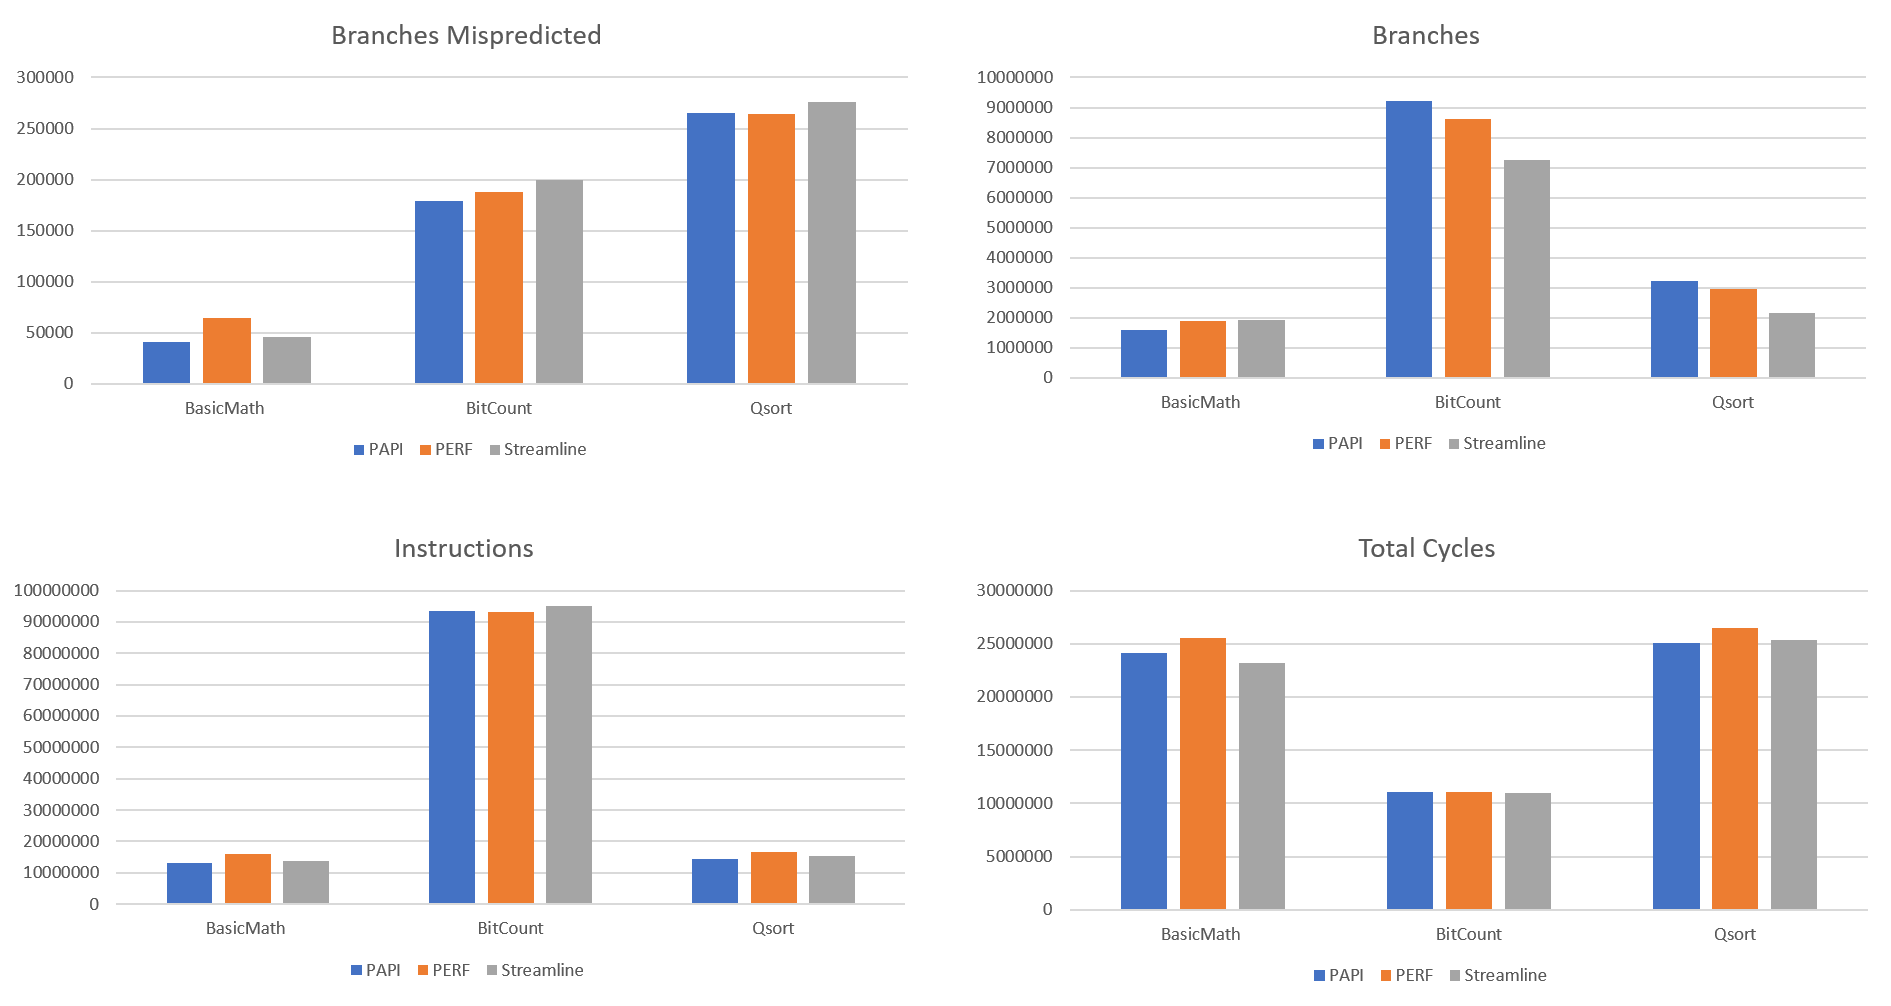
\includegraphics[width=14cm, height=14cm]{./images/tool_result}
\centering
\caption{Comparison of hardware performance counter values on PERF, PAPI and Steamline for BasicMath, BitCount and Qsort applications}
\label{fig:tool_results}
\end{figure}

\subsection{Tool selection}

We explored three performance measurement tools. We compared them with respect to parameters such as live analysis, annotations, API calls, Cost and etc. Also we compared the values captures by these tools on three different application with few hardware performance counters. All three tools have their own distinguish features such GUI for Streamline, Multiple counters at a time in PERF and API calls in PAPI. 

\par But most important hing is which is suitable for learning model. Because main objective of this thesis is to predict the performance. Which tools can be best fitted in this objective where performance data need to be collected at phase level of applications or software with LLVM tool chains. For that tool need to be have fast response time, easy to use and available free also. And most important, it should measure data at phase level. By considering all these factors, Streamline is slow in response and to collect large training data it will consume time and also it is paid. So Streamline can not be used here. Whereas PERF is open source tool, fast response but main disadvantage of PERF is that it is not able to measure performance data at phase level of software. And hence PAPI is best suitable tool to collect that performance data that can be used as training data. PAPI provides API calls that be inserted in phases of application using LLVM toolchain. Also response time is fast ans it is available free of cost.

\section{Grouping of the Counters}
In this thesis with respect to state of the art, we are going to see grouping of the hardware performance counters. Grouping of hardware performance counter is essential because in this thesis, we going to collect the training data in thirteen dimensional as input parameters and 1 dimensional output to understand the relationship between them. But measure concern is that total number of hardware performance counters available in PMU of Cortex A53 are 14. And we selected the tool for performance measurement is PAPI. PAPI allowed only 6 hardware performance counters to access at a time. So wee need to group hardware counters. 

\subsubsection{Multiple Measurements}
To test the PAPI as performance measurement tool, in this thesis work as small experiment, we used PAPI API calls in benchmark programs. In this experiment, we used PAPI high level calls in benchmark programs from MiBench[] and execute the same programs for 100 times to observe the consistency of values counted by PAPI tool for every execution. This data is gathered for complete program, not for different phases of programs. The following figure \ref{fig:grp_4} is resulted from execution of Basicmath program from MiBench benchmark suite. Program is executed 100 times and every time the total cycles, total instructions, level 2 cache miss, level 2 cache access, level 1 data cache miss and level 1 instruction cache miss, these hardware counters are measured for resulted figure. We also collected the data for other hardware counters for every execution and observed the consistency of PAPI tool in terms of performance measurement. 

\begin{figure}[h!]
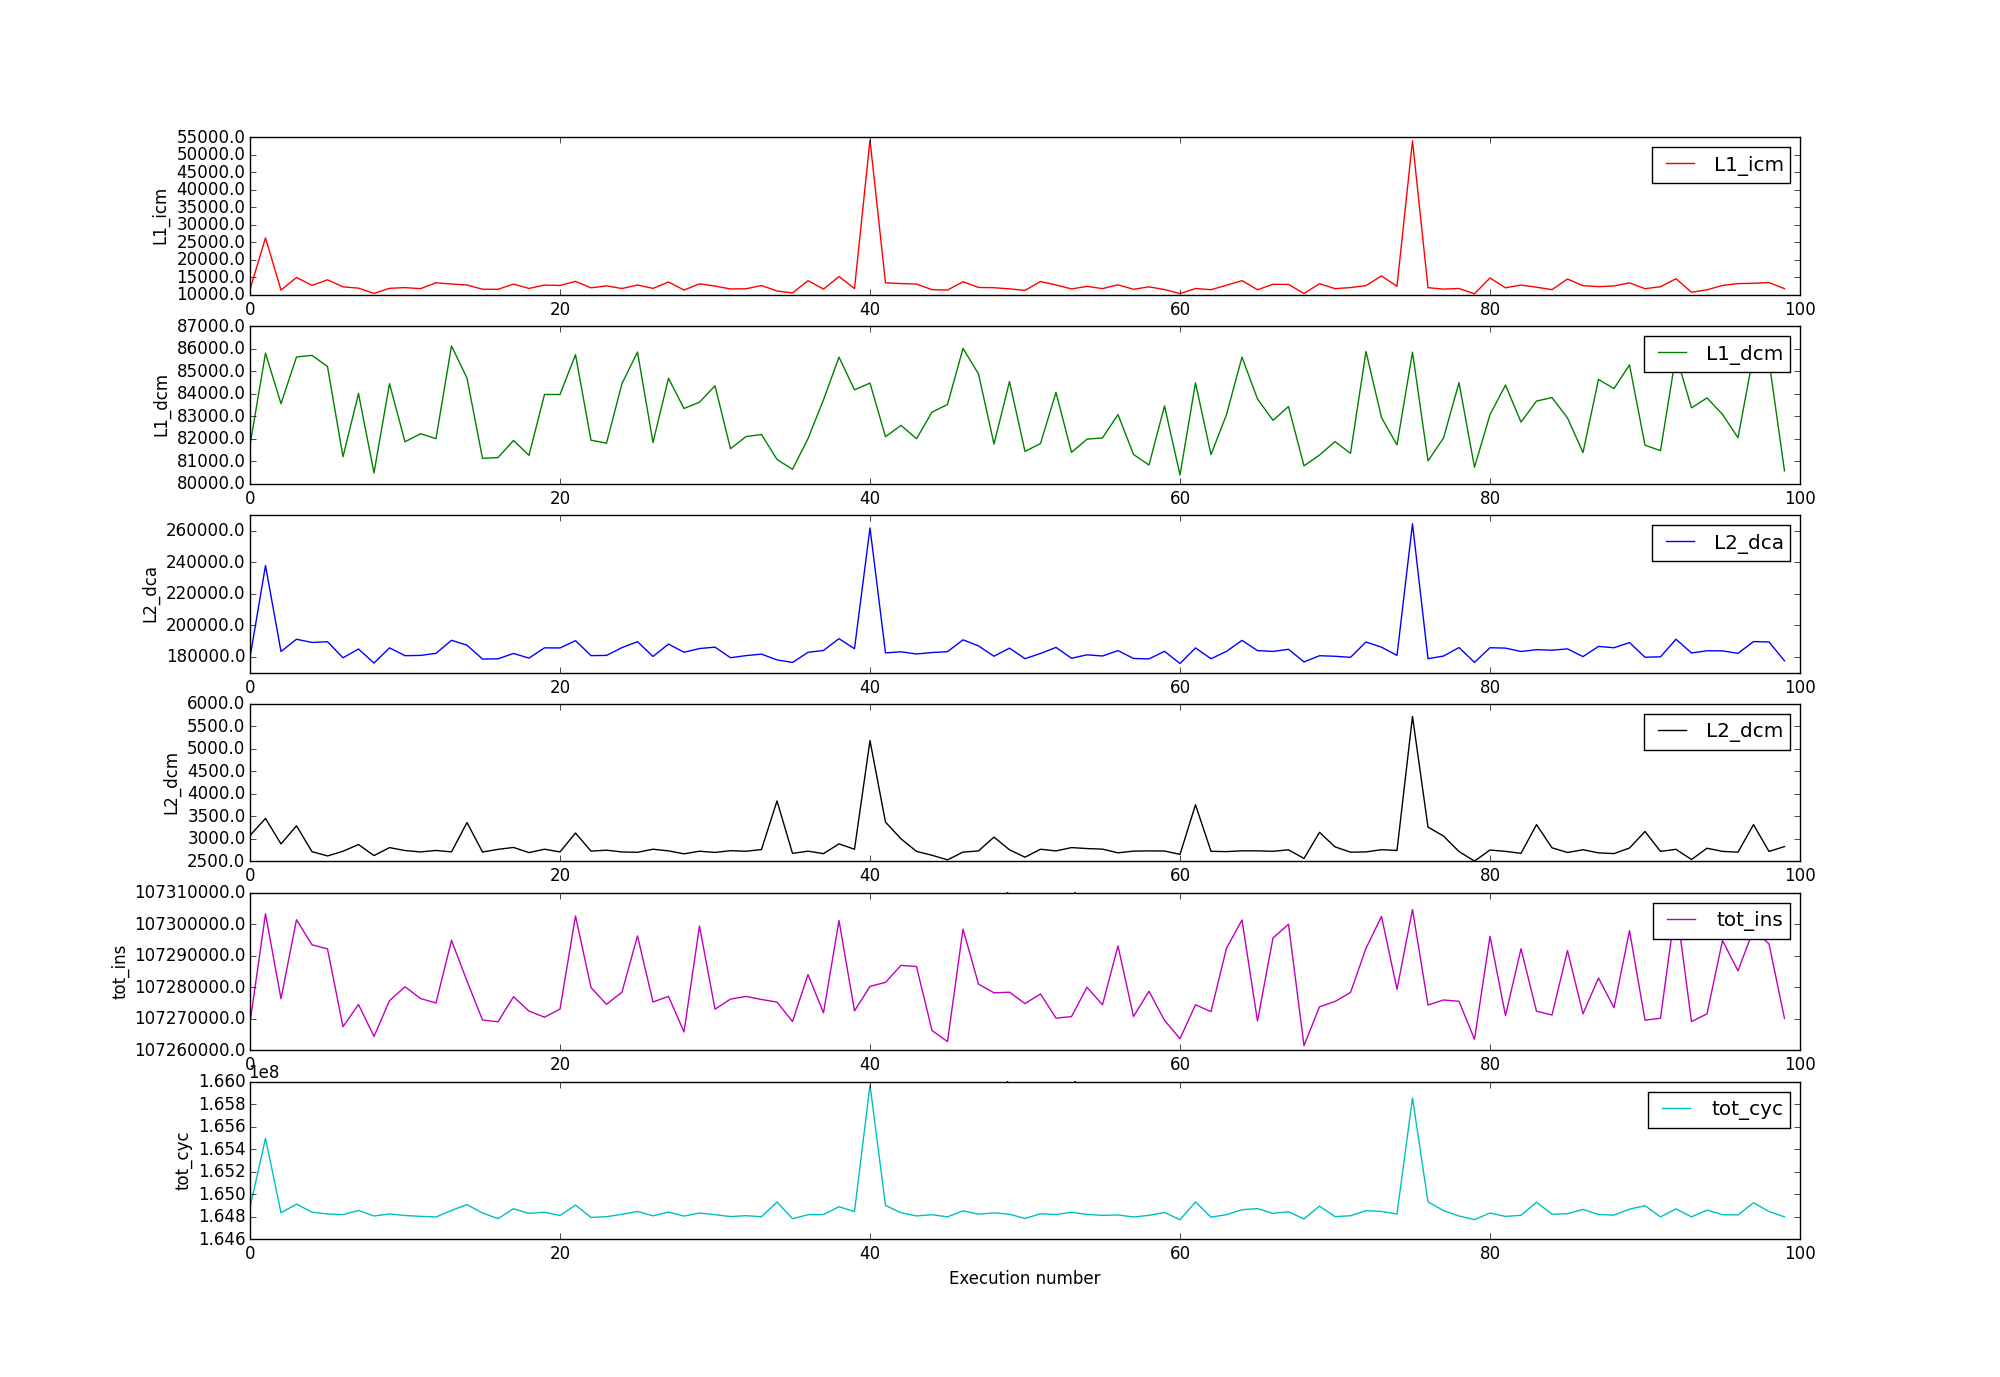
\includegraphics[width=14cm, height=14cm]{./images/grp_4}
\centering
\caption{100 time execution of same program using PAPI}
\label{fig:grp_4}
\end{figure}

\ we also calculated and plotted the percentage in hardware counter values with respect to average value. Following figure \ref{fig:grp_4_perc_change} shows the change in percentage for hardware counter discussed in above paragraph. As we can see the figure \ref{fig:grp_4_perc_change}, percentage change in hardware performance counter measurement is vary with respect microarchitectural events, but change is acceptable because there are might be some kernel process is active in background. While measurement we made sure to avoid external interruption during the measurement and measurements are taken on isolated core of Cortex A53.  

\begin{figure}[h!]
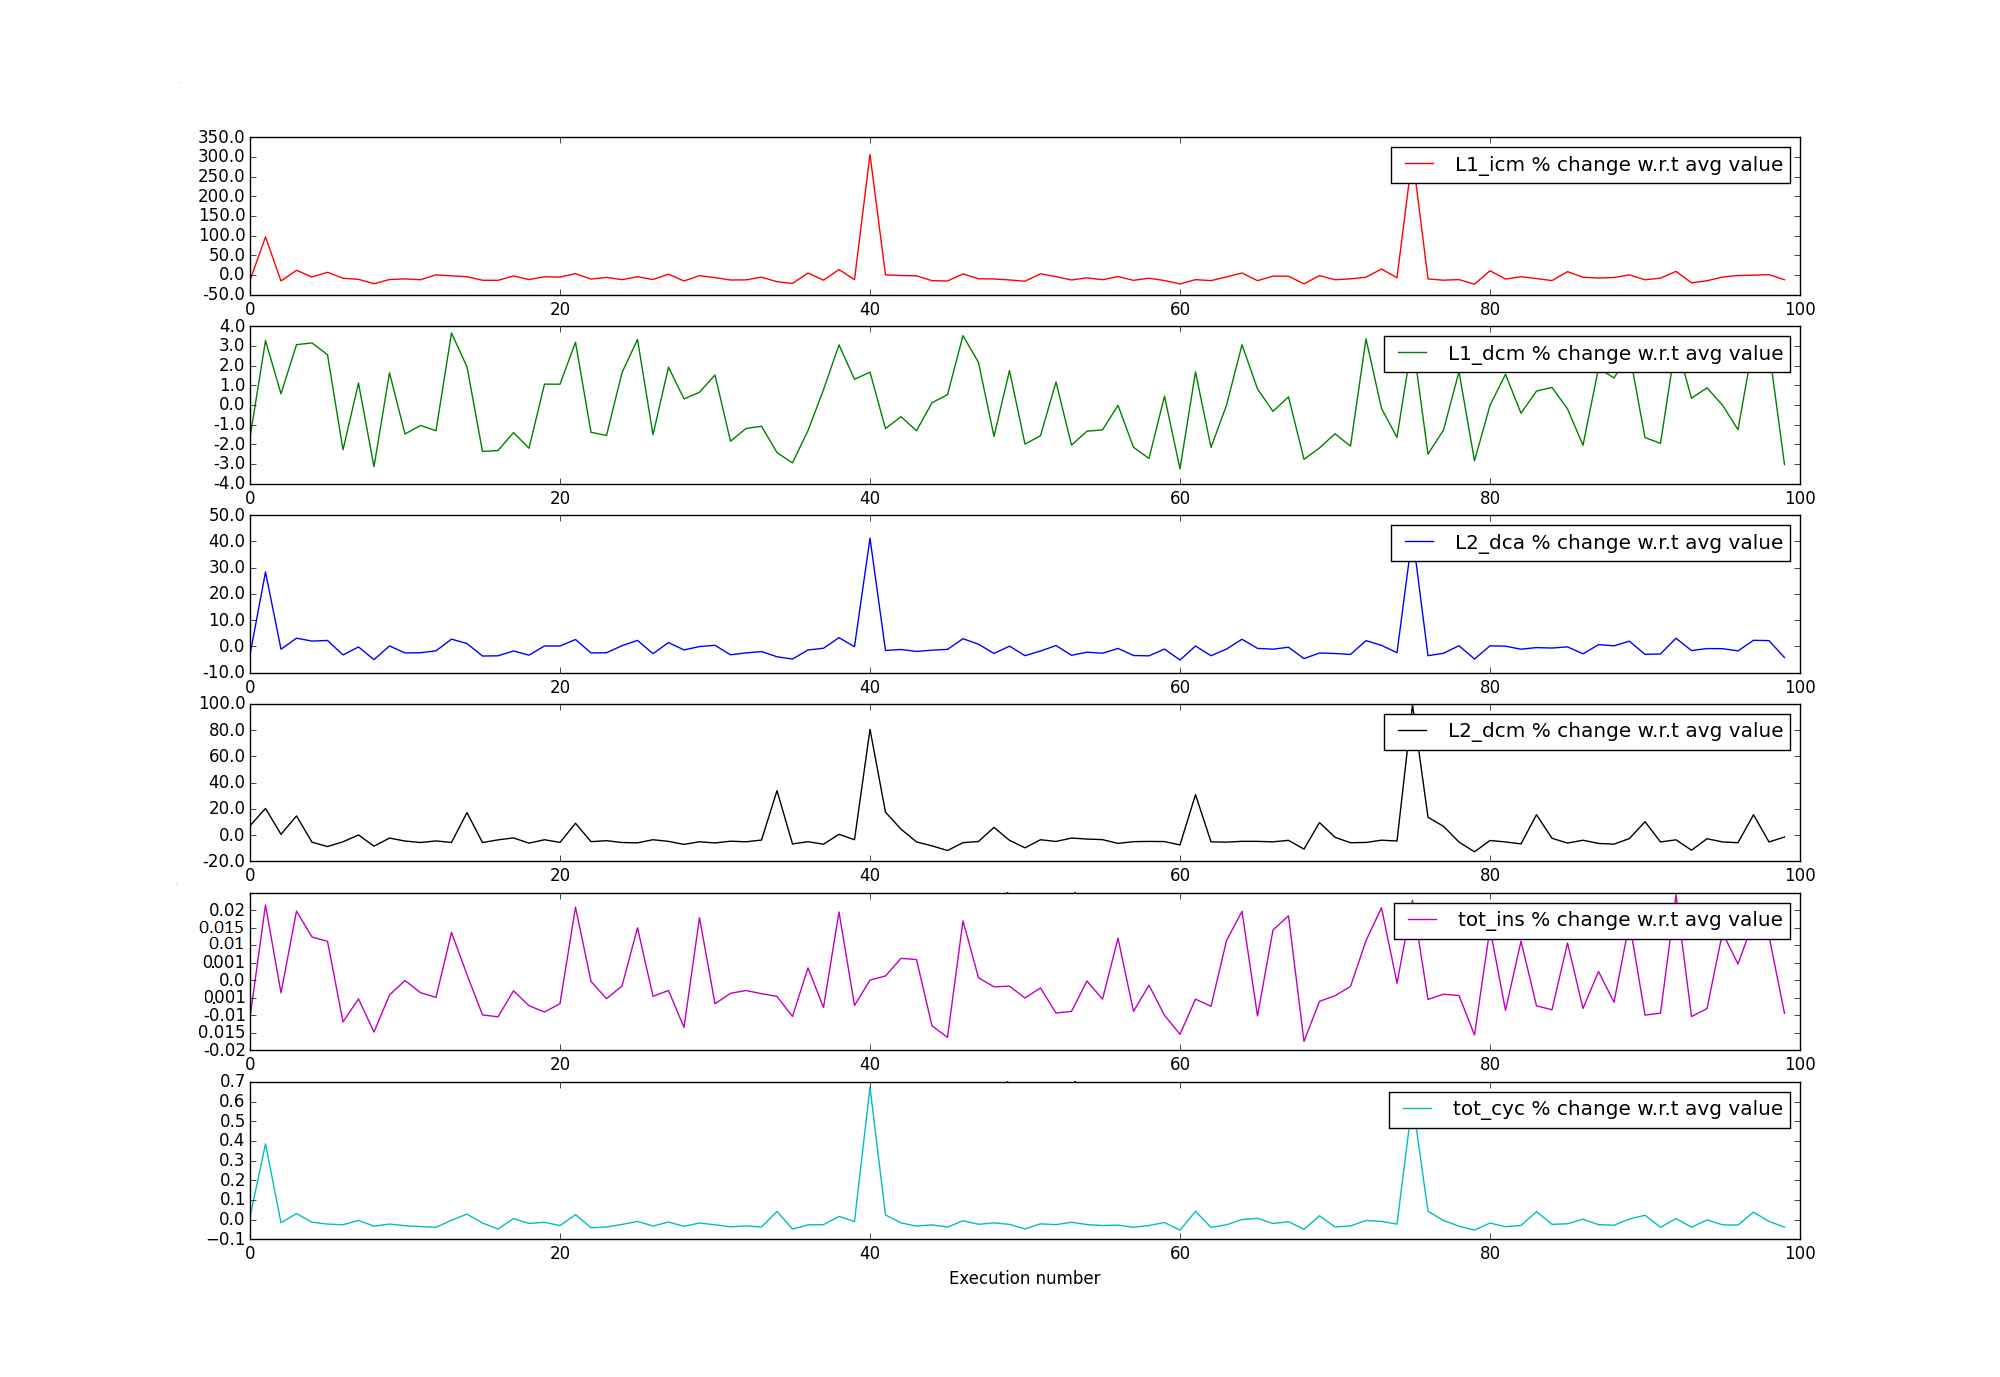
\includegraphics[width=14cm, height=14cm]{./images/grp_4_perc_change}
\centering
\caption{100 time execution of same program using PAPI}
\label{fig:grp_4_perc_change}
\end{figure}

\subsubsection{Counter grouping}
In order to observe the behavior of hardware counters on total cycles, we performed grouping of the hardware counters and number of hardware counters in each group are equal to 6 or less than 6 due restriction of accessing counters at a same time. In following table, you can see different combinations. These combinations are made in order to understand the impact of them on total number of cycles for same programs but with different groups.  We performed small experiment on Raspberry to conclude the final groups for hardware counter which are going to use in further processing like collecting training data and creating the framework. 

\begin{tabular}{|l|c|r|p{1.7cm}|}
  \hline
  \textbf{Sr. No.} & \textbf{Combinations}\\
  \hline
  1 & Branch instructions, Branch mispredicted, Total instructions, Hardware interrupts, L1 instruction cache miss, Total Cycles\\
  \hline
  2 & L2 data cache accesses, L2 data cache miss, Load instructions, Store instructions, Total cycles, Branch mispredicted\\
  \hline
  3 & TLB data miss, TLB instruction miss,  Branch mispredicted, L2 data cache miss, total cycles, Total instructions \\
  \hline
  4 & L1 instruction cache miss, L1 data cache miss, L2 data cache access, L2 data cache miss, total instructions, total cycles\\
  \hline
 5 & L1 instruction cache miss, L1 data cache miss, L2 data cache access, L2 data cache miss, Hardware interrupts, Total cycles\\
  \hline
  6 & L1 instruction cache miss, L1 data cache miss, L2 data cache access, L2 data cache miss, L1 data cache access, Total cycles \\
  \hline
  7 & Branch instructions, Branch mispredicted, Load instructions, Store instructions, Total cycles\\
  \hline
  8 & Hardware interrupts, TLB data miss, TLB instruction miss, Total cycles \\
  \hline
\end{tabular}


\par After running these combination of counters mentioned in above table are run on Raspberry for multiple time for multiple programs. While collecting the results, we monitored the impact of hardware counters on total number of cycles. From above combinations, we selected the combination 6,7 and 8. In combination of 6, we can see all hardware counters are related to caches. If level 1 cache is missed then it can be hit for level 2 or can be miss. By combining all cache related hardware counters, their impact can be understandable on cycles. Combination 7 consists, hardware counters related to instructions such as store instructions, load instructions, total instruction as well as total branches and branch mispredicted, their impact can be observed on cycles. Same time remained counters are grouped together for example, TLB instruction and data miss and hardware interrupts. These group does not have much impact oh cycles. 

\section{Application in Phase levels}
Collect the performance data at phase level is one the primary challenge in this thesis work. It is backbone of this thesis work. Performance data is collected at phase level of application on hardware platform. Which helps to understand the software behavior and the performance at different phases on hardware platform. In this thesis work, this main objective is accomplished with LLVM tool chain and PAPI library. This framework collect fine-grain level of data from application executing on hardware platform. Also with this framework, user can change the granularity of phases, which helps to understand the behavior at different granularity level. In this thesis work, we are using LLVM v3.5. 

\par LLVM is collection of reusable compiler and toolchain technology. It provides the toolchains like compiler, assembler, linker, optimizer, and etc. We are going to use Clang, native compiler from LLVM. It supports C/C++/Objective-C programming languages. It compiles faster than GCC compiler and provides useful warning and error messages. It also provide static analyzing of code to find bugs. We are also going to use LLVM linker, LLD, whichis helpful to link all bitcode files generated by Clang compiler. LLVM optimizer, opt, it takes input files and run specified optimizations and analysis on it. We are also going to use llc, that is LLVM's static compiler. Which compiles the source inputs into assembly language of specified architecture. 

\subsection{Creating phases}
Collect the data at phase level of application, PAPI libraries are used. These PAPI libraries are embedded into LLVM toolchain and shared objective library is created to divide application in different phases as well as in basic blocks. 


\subsubsection{Finding the basic blocks}
LLVM allows to create LLVM pass framework. Most of the compiler's parts are exists in LLVM passes. LLVM passes perform the transformation and optimizations that make up the compiler. LLVM passes are subclasses of LLVM pass, there are many subclases such as ModulePass, FunctionPass, BasicBlockPass and many more passes, which gives the more information to system about what pass does and how it can be combined with other passes. Before that lets go through the more information about basic blocks. Basic blocks is traight lines of code sequence which consists one entry point and one exit point and in between this there are statement/s.

Using LLVM passes and PAPI API calls, PAPIInstrument shared library is created. This is created with LLVM passes like FunctionPass, BasicBlockPass, ModulePass, and InstructionPASS. Most basic and solid part is to find the number of basic block. This library provide option 'bbtrace' which shows the number of basic block. We can show in following command and result. We used same code as we mentioned in above section i.e. decimal to binary code. To get the list of basic blocks, code is compiled with Clang compiler and bitcode file generated for the code.

\begin{lstlisting}
$ opt -load $(INS_LIB) -bbtrace -analyze < dec_to_bin.bc > bbstats.log
$ cat bbstats.log

Printing analysis 'Basic Block Trace':
0: alloca 3 br 1 call 2 store 2 
1: br 1 icmp 1 load 1 
2: add 1 br 1 load 1 store 1 
3: add 1 br 1 load 1 store 1 
4: ret 1 
\end{lstlisting}

Using LLVM optimizer bitcode is analyzed and optimized. INS\_LIB is path to the shared library PAPIInstrument. Which provide option '\-bbtrace' to get the basic block. LLVM count and displays all basic blocks based on IR representeation code. Above results are generated for IR code decimal to binary conversion. Bitcode file consists the IR code representation of the code. Using this IR code representation basic blocks are counted.

\subsubsection{Adding instrumentation calls}
Now, we know how to find basic blocks from applications. Now main task is to insert performance measurement API calls of PAPI in these blocks. To measure the performance of each basic block is not feasible. It can cause more overhead because PAPI API calls also going to be part of it while executing the application on hardware platform. So we decided to combine number basic block and we called it as phase. Phase consist number of basic blocks which user can defined. In diagram \ref{fig:phase} illustrate the phases. In this figure \ref{fig:phase}, one phase consist 1000 basic blocks. And we called it granularity of 1000. Granularity can be increased or decreased. Last phase may contains 1000 basic blocks or less than basic block because last phase consist only remaining basic blocks in it. 

\begin{figure}[h!]
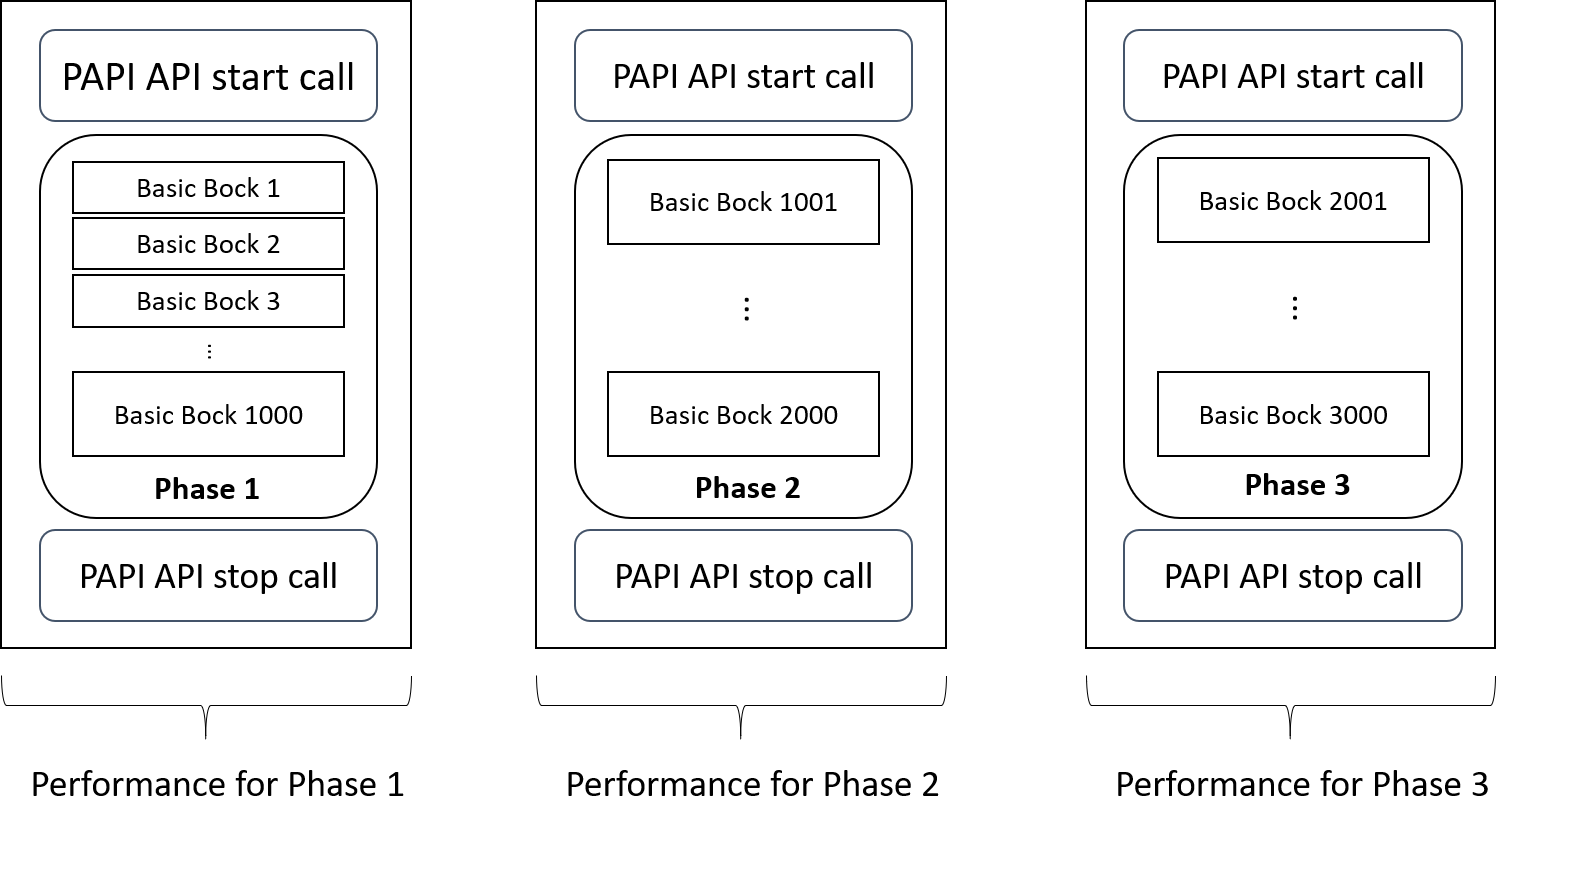
\includegraphics[width=13cm, height=10cm]{./images/phase}
\centering
\caption{Phases with granularity of 1000}
\label{fig:phase}
\end{figure}

\par Granularity of different sizes is possible due to PAPIInstrument library. Library combines the number of basic blocks based on defined granularity. For this it need additional source file of PAPI API calls to be linked with. First compiled code converted into bitcode and optimized using LLVM optimizer. PAPIInstrument library provide option 'papi\_instru\_bb'. This option need to be use while collecting performance at phase level. Following flow chart \ref{fig:flow} illustrate the creating phases and inserting performance call at start and i end of the phase. 

\begin{figure}[h!]
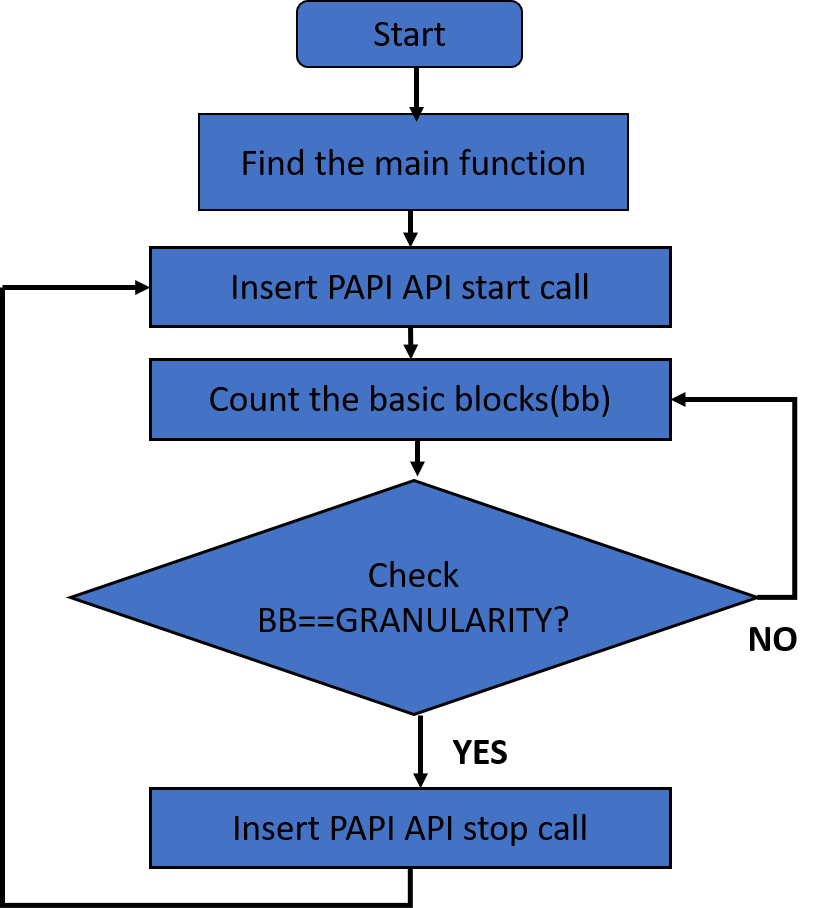
\includegraphics[width=10cm, height=13cm]{./images/flow}
\centering
\caption{Creating phases and adding performance calls}
\label{fig:flow}
\end{figure}

Followings are the instrumentation steps. All these steps are combined and composite into Makefile. This Makefile structure helps to create executable with single Linux command. INS\_LIB is the environmental variable which has the path of PAPIInstrument library set. 

  \textbf{Step 1: Compile the source files}
  \begin{lstlisting}
   $ clang -emit-llvm -g -I -c "source_file_name/s"
  \end{lstlisting}

In this step, LLVM compiler Clang compiles the source files which are written in C/C++ programming languages. Option \-emit\-llvm creates the bitcode file with .bc extension for each source file. 

  \textbf{Step 2: Link all bitcode files}
  \begin{lstlisting}
  $ llvm-link "source_files.bc" -o $(TARGET).linked.src.bc
  \end{lstlisting}

Step 2, uses llvm-link command from linker to link all bitcode files into single TARGET bitcode file. TARGET is name for executable gong to be created. Which will be single file resulted by linking all other bitcode files and that single file has local naming convention in this thesis work i.e. TARGET.linked.src.bc.

  \textbf{Step 3: }
  \begin{lstlisting}
  $ opt -load $(INS_LIB) -bbtrace -analyze < $(TARGET).linked.src.bc > bbstats.log
  \end{lstlisting}
  
  Step 3, Using optimzer and PAPIInstrument shared library, log file is created which has list of basic blocks. This step is optional. It only create log file of basic blocks. Instrumentation calls are not inserted during this step.
  
    \textbf{Step 4: }
  \begin{lstlisting}
  $ opt -load $(INS_LIB) -papi_instru_bb < $(TARGET).bc > $(TARGET).instru.bc
  \end{lstlisting}
  
  Step 4 adds instrumentation call at each phase level using PAPIInstrument library and create new bitcode file with .insru.bc extension with Target executable.

    \textbf{Step 5: }
  \begin{lstlisting}
   $ clang++ -emit-llvm -g -I $(PAPI_INC) -c papi_helper.cpp -o papi_helper.bc
  \end{lstlisting}
  
  In Step 5, bitcode for papi\_helper is created using Clang compiler. This papi\_helper consist the PAPI high level API calls. These API calls are going to inserted at each phase of the software or application of whos performance is going to collected.
  
 \textbf{Step 6: }
  \begin{lstlisting}
      $ llvm-link $(TARGET).instru.bc papi_helper.bc -o $(TARGET).linked.bc
  \end{lstlisting} 
  
  All bitcode files are linked using llvm linker like Target bitcode files with instrumentation call of bitcode of papi\_helper.  And single linked file is created with extension .linked.bc.
  
 \textbf{Step 7: }
  \begin{lstlisting}
$ llc -filetype=obj $(TARGET).linked.bc -o $(TARGET).o
  \end{lstlisting} 
  
  In Step 7, using LLVM static Compiler, LLC, which takes linked bitcode file as input and it compiled again with respect to target hardware architecture. It can be called object file and .o extension is given to compiled file with target executable name.
  
   \textbf{Step 8: }
  \begin{lstlisting}
 $ gcc $(TARGET).o -o $(TARGET) -L $PAPI_LIB -lpapi -lm
  \end{lstlisting} 
  
  Step 8 is the last step where executable for target is created. Where PAPI\_LIB is environmenatal variable consist path for PAPI libraries. 
  
\subsubsection{Automation to create Makefile}
All above steps are written in single makefile to create executable for single application. We have total 263 number of application from different domains and with single or multiple source files. To create makefile for each application can consume more time. So automation need to be created to make all makefiles. To execute each applications in this thesis work, it need at least 4 files. Source file, it can be either in C or C++, input file, in which consist all inputs for application which can be optional depends upon applications, Makefile and run executable to which contains the application executable. Also with each application we need papi\_helper file. We will see in coming section how to add the it using framework. 

\par We created two automation scripts using python and Linux Bash scripts. One automation screept is for single source file and another for multiple source files. Apart from that both have similar functionality. Both automation scripts removes the white spaces from source file names and create new name without white spaces. Renamed source file name is used as Target in makefile. These autotmation scripts make makefile for application with Target name as we discussed. These also create run executable file for Linux bash scripts which contains the target executable in it. These automation scripts are handy and less time consuming. 
  
\par Till now, we have seen PAPI tool and LLVM combination. And new PAPIInstrument library which creates the phases into application and insert performance measurement calls at start and end of phase. This is the backbone for upcoming frameworks, training and prediction framework.
  
\section{Framework to collect training data}
In this section, we are going to see framework which collects the training data with granularity. Prerequisite for this framework was grouping of hardware performance counters and instrumentation calls at phase level of applications. All these prerequisites are completed in previous session. One more thing, we need to understand is how granularity can effectively change with each group. 

\par As we discussed above, to insert instrumentation call at each phase, LLVM need papi\_helper file, which written in C++ programming language and it contains the granularity level as well as group of hardware counters. We have three groups of hardware counters and execution of same program need to be done three times with same granularity. For that we inserted automation script which is created using python. This scripts takes the hardware counter group and granularity as input. For example you can see it in following bash script. 

\begin{lstlisting}
#!/bin/bash

PAPI_EVENTS_BATCH_1=(PAPI_L1_DCM PAPI_L1_ICM PAPI_L2_DCM PAPI_L1_DCA PAPI_L2_DCA )
PAPI_EVENTS_BATCH_2=(PAPI_BR_MSP PAPI_BR_INS PAPI_TOT_INS PAPI_LD_INS PAPI_SR_INS)
PAPI_EVENTS_BATCH_3=(PAPI_TLB_DM PAPI_TLB_IM PAPI_HW_INT)

python $PY_UTIL/papi_helper_setup.py  ${PAPI_EVENTS_BATCH_1[@]} --granu 1000
python $PY_UTIL/papi_helper_setup.py  ${PAPI_EVENTS_BATCH_2[@]} --granu 1000
python $PY_UTIL/papi_helper_setup.py  ${PAPI_EVENTS_BATCH_3[@]} --granu 1000

\end{lstlisting}

This bash scripts uses python script i.e. papi\_helper\_setup.py to create papi\_helper file, which is going to use for instrumentation of applications. Path of the automation script is stored in environmental variable PY\_UTIL. This script uses template script to create papi\_helper with given hardware counters and granularity. Script require to input parameters. One is list of hardware performance counters and granularity in integer number. 

\par Now we will see the use of the training data framework. All application with makefile and run executables are store in training\_programs repository. Framework to collect training data has the path for training application repository stored. Another important change need to be made in framework is that whether user want to collect the training data on single core or on dual core with no load or full load. Following command can be use for single core and dual core modes. In dual core scenario, data is collected in two different environment. 
\begin{itemize}
\item[$\bullet$] No load
\item[$\bullet$] Full load
\end{itemize}

This command is for single core mode. Where core 2 is isolated and using this command user can force applications to execute on core 2.
\begin{lstlisting}
$ sudo taskset -c 2 ./run
\end{lstlisting}

Following command can use to collect the data on dual core. 
\begin{lstlisting}
$ sudo chrt -r 1 taskset -c 2,3 ./run
\end{lstlisting}

\textbf{No load}
\par In no load scenario, no background additional process is running. Only operating system is running on it i.e. Raspbian. Other two core, core 0 and core 1 are isolated from execution. Only core 2 and core 3 are active. All performance data is collected on these two cores. using framework. 

\textbf{Full load}
\par In full load scenario, same prerequisites are applied. Core 0 and core 1, are isolated and all operations are performed on core 2 and core 3. To make it full load scenario, background application is running on core 3. We use stream application[] to utilize the core 3. Application try to utilize core 3 completely in background and same time training data is collected from both core for training programs. 

\par We saw insights of the training phase framework.  All the Linux commands and automation commands are combined into single bash script. And this bash script can start the framework with input parameter as integer number represent the granularity. We can start the framework with following commands in command prompt with granularity of 1000. But before starting the framework, make sure that all environmental variables are set. 

\textbf{Single core}
This is the bash script to start single core collection of training data.
\begin{lstlisting}
$ ./auto_exec_single_core 1000
\end{lstlisting}

\textbf{Dual core}
This is the script to start dual core collection of training data but same time in full load mode background application needs to be started on core 3. 
\begin{lstlisting}
$ ./auto_exec_dual_core 1000
\end{lstlisting}

\par All the performance data collected stored in input.dat and ouput.dat file. Data related to hardware performance counters except cycles is stored into input.dat file where total number of cycles are stored in output.dat file. These files contains all training data collected from all 263 training programs which can be feed to machine learning algorithms. 


\section{Data Analysis}
Previously, we saw training phase framework, which collects the data from training data on single core as well as dual core. Training data collected from 263 application programs which is big in terms of hundreds of Megabytes. To understand the behavior of the training data and to decide which learning algorithm can be applied, are decided from analyzing the training data known as data analysis techniques. Data analysis process examines the data which helps to draw the conclusions about information contains in data. Data analysis techniques are used in commercial industries, research filed, and many more. 

\par Data analysis techniques provides procedures for inspection, cleansing, transforming and modeling the data which supports in decision-making. These techniques process raw data and convert it into useful information. In this thesis, we are going to use to techniques, those are, Principal Component Analysis(PCA) and correlation coefficient. Training data is fed to these techniques as raw data to collect useful information and decide the which learning model should be used. 

\subsection{PCA}
PCA technique is used for data exploration and visualization. Visualizing data provide more information to analytic about relationship between variables. We can plot and visualize data till 3 dimension but what if we have variables more than 3 dimensions. In such cases it not possible to visualize the data if data has more variables. Also having number of variable more in data can cause overfitting to learning model to data.

\par Taking all variables and focus on only few data is possible with PCA. PCA allows the reduction in the dimension of the data. By reducing the dimensions of feature variables, which allows to consider fewer relationship between variables and learning model likely to overfit your model. Reducing the dimensions of the feature space is called dimensionality reduction. PCA can use to reduce the number of variables, ensure the variables are independent and to make the independent varibale less interpretable. 

\par PCA finds the principal component of data. It is useful to measure data in terms of principal components rather than x-y axis. Principal components are underlying structure in data. They are the directions where there is most variance is. The directions where data is mostly spread out. Instead of using x-y-z axis cordinates to observe or monitor the data, PCA uses principal components. These principal components can use for analyzing the data as well for visualizing the data. 

\par To find the variance PCA uses eigenvectors and eigenvalues. Eigenvectors and eigenvalues are exist in pairs that means every eigenvector has corresponding eigenvalue with it. Where eigenvector is direction and eigenvalue is number which provides the information about variation in data in that direction. The eigenvector with highest eigenvalue is principal component. For every dimension, there is one eigenvector and eigenvalue associated with it. for example two dimensional data have two eigenvectors and eigenvalues. Using PCA we get new axis which provide information about more variation in direction. 

\par In this thesis PCA is used for dimension reduction. We reduce dimension from 14D to 2D. Reducing the dimensions helps to simplify the data and makes it easier to visualize. We are using sklearnn[] libraries of python to apply PCA on training data. Here, user can choose the two highest eigenvectors which are calculated from multidimensional data. Those two eigenvectors with eigenvalues are the principal components. These principal components can be visualize by plotting them like x-y axis. PCA  helps to reduce the dimensionality of data and that data can be visualize to understand the behavior of the data collected and to draw furhter conclusions. 

\par In this thesis work, we used PCA techniqu on single core as well dual core for both scenarios. We collected the training data for 15 different granularity and we applied PCA to these different granularity of the training data. In following figures, you can see PCA for single core, dual core no load scenario and dual core full load scenario. 

\begin{figure}[h!]
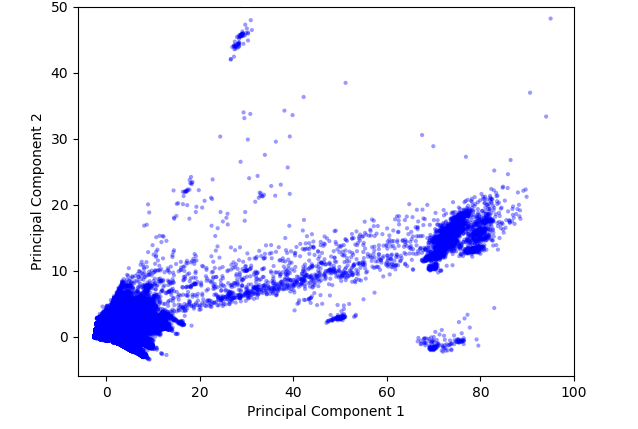
\includegraphics[width=12cm, height=8cm]{./images/single_core_pca}
\centering
\caption{PCA for single core at granularity of 1000}
\label{fig:flow}
\end{figure}

\begin{figure}[h!]
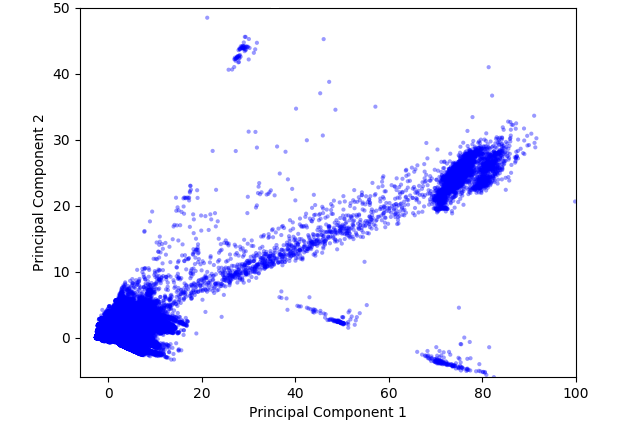
\includegraphics[width=12cm, height=8cm]{./images/dual_no_pca}
\centering
\caption{PCA for dual core with no load at granularity of 1000}
\label{fig:flow}
\end{figure}

\begin{figure}[h!]
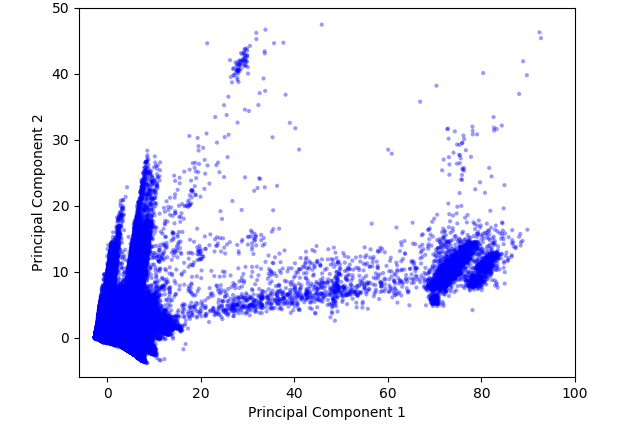
\includegraphics[width=12cm, height=10cm]{./images/dual_full_pca}
\centering
\caption{PCA for dual core with full load at granularity of 1000}
\label{fig:flow}
\end{figure}


\subsection{Correlation Coefficient}
Correlation is widely used statistical concept. Term correlation indicate to mutual relationship between variables or quantities. It is first step to understand the relationship in variables of data. Correlation can indicate or provide information about relationship between variable whether it is casual or intense with other variables. Correlation coefficient provides numerical measure of statistical relationship between two variables. 

\par There are different mathematical techniques are available to calculate correlation coefficient. Such as Pearson technique, Spearman technique, Kendall's Tau technique and many more. In this thesis work we are using Pearson technique. In this thesis work we going to use Pearson technique. We used sklearn[] library from python to calculate correlation coefficient and plot the correlation between each variable. 

\par Values of correlation coefficient for Pearson technique lies between -1 to +1. +1 indicate strongest positive linear relationship whereas -1 indicates the strongest negative linear relationship. We calculated correlation for each hardware performance counter with respect to total cycles to understand the relationship of each of them with total cycles. We calculated correlation coefficient for single core, dual core with no load and dual core with full load for 15 different granularities of training data. We also plotted the heatmap to visualize the relationship of each each hardware counter with other hardware counters i.e. 14x14 correlations. 

\par Following diagrams are correlation coefficient of  training data from single core, dual core with no load and dual core with full load.

\begin{figure}[h!]
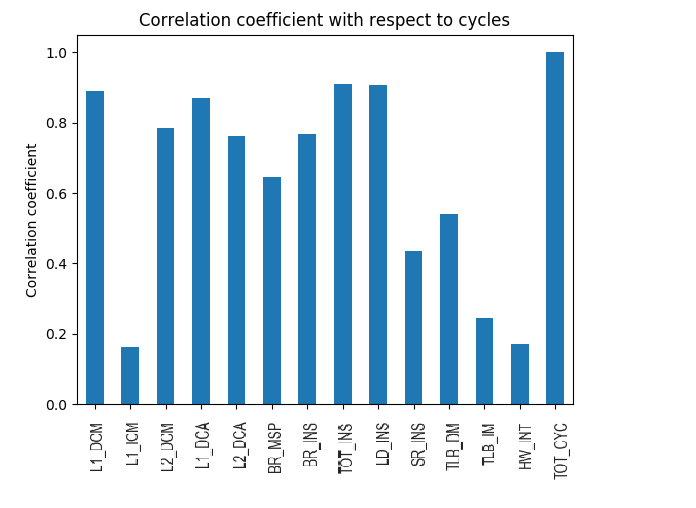
\includegraphics[width=12cm, height=8cm]{./images/CC_single}
\centering
\caption{Correlation coefficient with respect to total cycles on single core}
\label{fig:flow}
\end{figure}

\begin{figure}[h!]
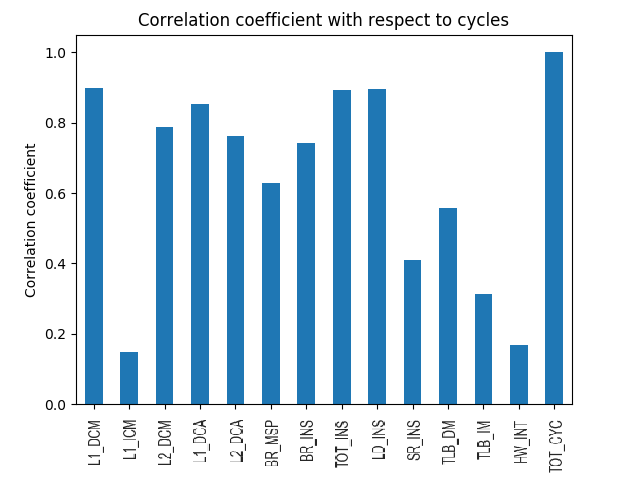
\includegraphics[width=12cm, height=8cm]{./images/CC_no_load}
\centering
\caption{Correlation coefficient with respect to total cycles on dual  core with no load}
\label{fig:flow}
\end{figure}

\begin{figure}[h!]
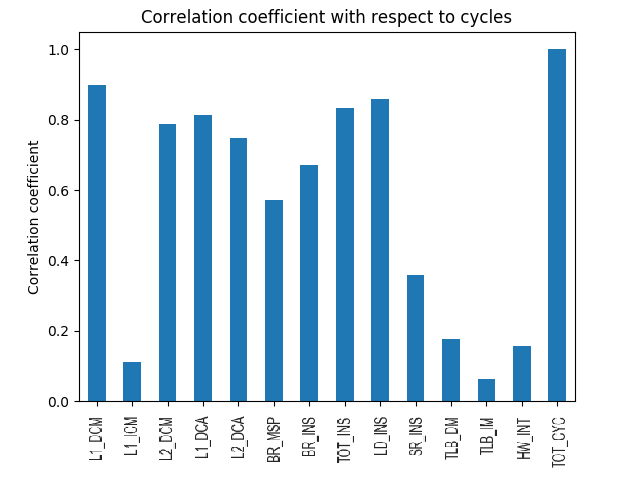
\includegraphics[width=12cm, height=8cm]{./images/CC_full_load}
\centering
\caption{Correlation coefficient with respect to total cycles on dual  core with full load}
\label{fig:flow}
\end{figure}

\begin{figure}[h!]
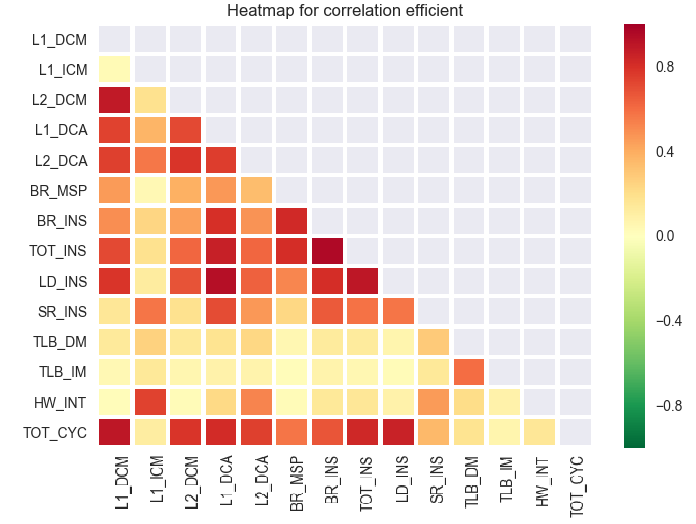
\includegraphics[width=12cm, height=8cm]{./images/heatmap_full_load}
\centering
\caption{Correlation coefficient heatmap for all hardware counters with respect to each other on dual core with full load scenario}
\label{fig:flow}
\end{figure}

\subsection{Hyposthesis of data analysis}
In above section, we saw the two data analysis techniques which are used in this thesis work on training data collected from single core and dual core for both scenarios with 15 different granularities. Visualization of data helps to understand the data and provide more information to draw conclusions for further procedures. 

\par Using PCA, we reduced the data into 2 dimensions and able to relate the data in 2D. Whereas using correlation coefficient, we understood the relationship of each counter with total cycles. Which draws the conclusion that relationship is linear. We can use supervise learning models to predict the performance in terms of cycles. Supervised learning maps input to an output based on input-output pairs. We are going to use 13 dimensional hardware counter data as input and cycles as output. 

\section{Prediction Framework}

 In prediction phase, we are going to use second framework that is prediction framework.  Prediction framework has same structure as training framework to collect the performance data. In addition to training framework, learning model is used to predict the performance of programs. In this framework, training data is used to learn the models. In training data, we have 13 independent variables and single dependent variable. These regression estimates the relationship multiple independent variables and single dependent variable. As our data behavior is linear, we are going to use supervise linear learning techniques like variants of linear regressions. There many learning models are available for linear regression. Following figure \ref{fig:prediction} illustrate the prediction framework. 

\begin{figure}[h!]
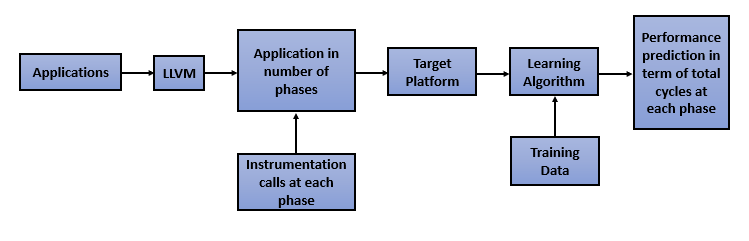
\includegraphics[width=14cm, height=5cm]{./images/prediction}
\centering
\caption{Prediction framework}
\label{fig:prediction}
\end{figure}

After collecting the training data for all hardware counters from 263 training programs, our essential goal is to form a mapping between them in such a way that if new performance data is collected then this mapping can help to estimate the cycles in terms of performance. For given \textit{d}-dimension, $x \in \mathcal{R}^d$ is performance feature vector obtained from host platform and its corresponding timing reference $y \in \mathcal{R}$ is also obtained from hardware platform then mapping function or model ${R}^d$ \textrightarrow ${R}$ is given by , 

\begin{center}
$f(x)=y$
\end{center}

In this section, we are going to discuss the choice of the $f$. We are going to see different variants of linear regression such as Lasso regression, Ridge regression and CLSLR model. 

\subsection{Lasso Regression}
LASSO is acronym for Least Absolute Shrinkage and Selection Operator. The full form of Lasso gives us hint that it is type of linear regression that uses shrinkage. Data values are shrunk toward to mean point. Lasso is simple model with fewer parameters. This model is used for data fitting technique. Objective of lasso is to find the subset predictors that minimizes the prediction error. 

First, lets see the basic linear regression model can be formulated by following equation, where given data set has $n$ points $(x_{i},y_{i})$, for $i = 1,...n$.

$ minimize \theta,   J(\theta) = || X \theta -Y ||^{2 }$ 

Where, $X \in \mathcal{R}^n \times d$ is rows of matrix with $d$ dimensional feature vectors $x_{i}$ and $y \in \mathcal{R}^n$ is column vector $y_{i}$ corresponds to each $x_{i}$. The model $f$ is said to linear when $f(x)=x^{T}\theta$ . such problem is also known as ordinary least square problem.


\par Lasso regression uses L1 regularization. L1 regularizations adds penalty to absolute value of coefficients magnitude. Which can be result in fewer coefficients because some coefficients can become zero and eliminated from the model.  Larger the penalty, closer the value of coefficients to zero which provides simpler model. Goal of the algorithm is to minimize, 

$minimize \theta,  J(\theta)=\dfrac{1}{2n} || X\theta - Y||^{2} + \lambda||\theta||$


Where, $X \in \mathcal{R}^n \times d$ is rows of matrix with $d$ dimensional feature vectors $x_{i}$and $y \in \mathcal{R}^n$ is column vector $y_{i}$ corresponds to each $x_{i}$. The function $f$ remain linear. As we can see in equation is that only difference between ordinary and lasso regression problem is L1 penalty applied to parameter $\theta$. This penalty restrict the $\theta$ to sparse. 

\subsection{Ridge Regression}
Ridge regression is a way to create simple model when number of independent variables are more than predicting or depending variables. Least regression model allows all independent variables regardless whether they are important or not important, which might leads to overfitting of the model and failure to unique solutions. Ridge regression avoid all these problems. 

\par Like lasso regression, ridge regression also uses shrinkage method. Here it uses shrinkage estimator called ridge estimator. Also ridge regression belongs to class of L2 regularization which adds L2 penalty. L2 penalty is equal to square of the magnitude of coefficients. All coefficients are shrunk by same factor so none are eliminated in model. Whereas L1 regularization leads model to be more sparse which is eliminated in ridge regression due to L2 penalty. 

\par Tuning parameter $\lambda$ controls the penalty, if $\lambda = 0$ then ridge regression is similar to least square regression or normal linear regression. When $\lambda = \infty$then all coefficients are shrunk to 0. So ideal value of penalty lies between 0 and $\infty$. Goal of the ridge regression is to minimize $\theta$,

$minimize \theta,  J(\theta)=\dfrac{1}{2n} || X\theta - Y||^{2} + \lambda||\theta||^2$ 

Where, $X \in \mathcal{R}^n \times d$ is rows of matrix with $d$ dimensional feature vectors $x_{i}$and $y \in \mathcal{R}^n$ is column vector $y_{i}$ corresponds to each $x_{i}$. Difference between ridge regression and other regression is that L2 penalty is applied to $\theta$. $\lambda$ is tuning para meter which can change the L2 penalty for model. 

\subsection{Constrained Locally Sparse Linear Regression (CLSLR)}
Assuming the relationship between variables is linear, lasso and ridge regression are expected to have good performance. But if the relationship is non linear then performance of model can suffer. To deal with this issue CLSLR can be used. In CLSLR, L1 penalty is introduced for finding the sparse solution of parameter $\theta$.

\par CLSLR uses euclidean distance between to two unit vectors. The distance $d$ can defined by distance between any two input feature points $x_{i}$ and $x_{j}$ as follows, 

$ d = || \frac{x_{i}}{||x_{i}||} - \frac{x_{j}}{||x_{j}||} ||$

CLSLR solves following optimization problem, 

$minimize \theta_{x_{t}},  J(\theta_{x_{t}})=\dfrac{1}{2m} || X_{x_{t}}\theta_{x_{t}} - Y_{x_{t}}||^{2} + \lambda||\theta||$

where each row $x_{i}$ of the matrix $X_{x_{t}}$ and each row of $y_{i}$ of the matrix $Y_{x_{t}}$ corresponds to points $(x_{i},y_{i})$ in neighborhood $N_{x_{t}}$ with respect to input vector $x_{t}$. CLSLR identifies the $m$-nearest neighbor of $x_{t}$ and solve optimization problem using above equation and obtain $x_{t}$ and compute the prediction by, 

$y_{t} = x_{t}^{T}\theta_{x_{t}}$

\par In prediction phase, performance data is collected and given as input to these algorithm to predict the cycles. These learning algorithms use training data to learn the relationship or mapping the relationship between independent and dependent variables to predict the performance for input data. 





  % Load Data from File intro.tex
%------------------------------------------------------------------------------
% Chapter 7 : Results and Discussion
%------------------------------------------------------------------------------
\chapter{Future Outlook}
% ------------------------------------------------------------------------------
% Chapter 7 : Future Outlook
% ------------------------------------------------------------------------------
TBD  % Load Data from File intro.tex
%------------------------------------------------------------------------------
% Chapter 8 : Summary and Outlook
%------------------------------------------------------------------------------
\chapter{Conclusion}
% ------------------------------------------------------------------------------
% Chapter 8 : Conclusion
% ------------------------------------------------------------------------------
TBD  % Load Data from File intro.tex
%------------------------------------------------------------------------------

%\chapter{Tables}
%% Example of, how to use a Table

\blindtext[1]

\begin{center}
\begin{tabular}{|c|c|c|c|}
\hline
Wert 1 & Wert 2 & Wert 3 & Wert 4\\
in Einheit1 & in Einheit2 & in Einheit3 & in Einheit4 \\
\hline
192 & 80& 0.3153 & 0.4900\\
500 & 120& 0.1229& 0.1787\\
1000 & 120& 0.0680& 0.0880\\
2000 & 120& 0.0361& 0.0441\\
5000 & 140& 0.0256& 0.0305\\
5000 & 164& 0.0343& 0.0880\\
\hline
\end{tabular}
\captionof{table}{This is the caption of the table}
\label{tab:table1}
\end{center}

\blindtext[3] % Load Data from File example_tables

%\chapter{Figures}
%% Example of, how to use figures

\blindtext

\begin{figure}[h]
\centering

\includegraphics[width=0.6\textwidth]{TU_Chemnitz_positiv_gruen.pdf}
\caption{Graphic 1}
\label{fig:pic0}
\end{figure}

\blindtext
\blindtext

\begin{figure}[h]
    \subfigure[This is the first graphic]{
\includegraphics[width=0.49\textwidth]{TU_Chemnitz_positiv_gruen.pdf} \label{fig:pic1}}
    \subfigure[This is the secound graphic]{
\includegraphics[width=0.49\textwidth]{TU_Chemnitz_positiv_gruen.pdf}\label{fig:pic2}}
\caption{This is the caption of the whole graphic}
\end{figure}

\blindtext

 % Load Data from File example_figures

%\chapter{Referencing}
% Alternativ just write your text under \chapter like this example

%\blindtext \cite{autorenrichtlinien}

%\blindtext \footnote{Here is an area for your Notes}

%\blindtext \footnote{\cite{lnilatex} Seite 11}
%\blindtext \cite{lnilatex}
%\blindtext \cite{autorenrichtlinien,pepper1992grundlagen,chen2001audiovisual}
%\blindtext \cite{ChelseaFC}

%\chapter{Subchapter}

%\section{sub 1}
%\blindtext[3]
%\section{sub 2}
%\blindtext[3]
%\subsection{sub 2.1}
%\blindtext[3]

%\subsection{sub 2.2}
%\blindtext[3]

%------------------------------------------------------------------------------
% bibliography based on Springer Design
%------------------------------------------------------------------------------

\bibliographystyle{splncs03}
\bibliography{bibliography}

\printindex

%------------------------------------------------------------------------------
% List of Abbreviations
%------------------------------------------------------------------------------
\twocolumn
\addchap{List of Abbreviations}

\begin{acronym}
	
	\acro{API}{Applicaton Program Interface}
	\acro{ASIL}{Automotive Safety Integrity Levels}
	\acro{BPF}{Berkeley Packet Filter}	
	\acro{Bash}{Bourne-again shell}
	\acro{BIOS}{Basic Input/Output System}
	\acro{BLOB}{Binary Large Object}
	\acro{BMP}{Bitmap}
	\acro{CISC}{Complex Instruction Set Computing}
	\acro{CPU}{Central Processing Unit}
	\acro{DLL}{Dynamic Link Library}
	\acro{DMA}{Direct Memory Access}
	\acro{DOS}{Disk Operating System}
	\acro{DRAM}{Dynamic Random Access Memory}
	\acro{eBPF}{Linux Enhanced BPF}
	\acro{FIDL}{Fuchsia Interface Description Language}
	\acro{FTP}{File Transfer Protocol}
	\acro{GPU}{Graphics Processing Unit}
	\acro{GUI}{Graphical User Interface}
	\acro{GUID}{Globally Unique Identifier}
	\acro{IDE}{Integrated Development Environment}
	\acro{IP}{Internet Protocol}
	\acro{IPC}{Inter Process Communication}
	\acro{ISO}{	International Organization For Standardization}
	\acro{KDE}{K Desktop Environment}
	\acro{KOID}{Kernel Object ID}
	\acro{LK}{Little Kernel}
	\acro{MBR}{Master Boot Record}
	\acro{OS}{Operating System}
	\acro{QEMU}{Quick Emulator}
	\acro{RAM}{Random Access Memory}
	\acro{RTE}{Runtime Environment}
	\acro{SDK}{Software Developement Kit}
	\acro{SSH}{Secure Shell}
	\acro{SSL}{Secure Sockets Layer}
	\acro{TOML}{Tom's Own Minimal Language}
	\acro{VM}{Virtual Machine}
	\acro{UDP}{User Datagram Protocol}
	\acro{URL}{Uniform Resource Locator}
	\acro{VGA}{Video Graphics Array}
	\acro{VPI}{Virtual Path Identifier}
	\acro{vDSO}{Virtual Dynamic Shared Object}
	\acro{WIP}{Work in Progress}
	
\end{acronym}
\onecolumn
%------------------------------------------------------------------------------
%List of Figures
%------------------------------------------------------------------------------
\listoffigures
%------------------------------------------------------------------------------
%List of Tables
%------------------------------------------------------------------------------
\listoftables
%------------------------------------------------------------------------------
% Appendices
%------------------------------------------------------------------------------

\begin{appendices}

%------------------------------------------------------------------------------		
\chapter{AAAA}
% ------------------------------------------------------------------------------
% Appendix  A : Fuchsia
% ------------------------------------------------------------------------------
TBD
%------------------------------------------------------------------------------
\chapter{BBBB}
% ------------------------------------------------------------------------------
% Appendix  B : Redox
% ------------------------------------------------------------------------------
TBD
%------------------------------------------------------------------------------	
\chapter{Performance Evaluation}
% ------------------------------------------------------------------------------
% Appendix  C : Performance Evaluation
% ------------------------------------------------------------------------------
TBD
%------------------------------------------------------------------------------		
			
\end{appendices}

\end{document}


